\section{P\'olya's Bessel function: hitting times, a clock and the flow}\label{ch:biane}

P\'olya replaced the kernel $\Phi$ of \eqref{eq:ch2:Phi} by its asymptote $\Phi^*$ and proved that the transform $\Xi^*$ has only real zeros \cite{Polya} (Section~\ref{fm:sec:simple}). The building block of his proof is the Macdonald function
\begin{equation}\label{eq:biane:P}
P(\theta)=K_{i\theta/2}(2\pi)=\int_{\R}e^{-2\pi\cosh2u}\,e^{i\theta u}\,du,
\end{equation}
which has only real zeros and whose zero counting function has the main term of the Riemann von Mangoldt formula. Biane \cite{Biane09} showed that $\Xi$ and $P$ are Mellin transforms of two Brownian hitting times, and that the Thorin measures of these hitting times are spectral measures of the radial Brownian motions on the unitary group $SU(2)$ and on the hyperbolic space $SL_2(\C)/SU(2)$. This section follows the first author's note on Biane's paper \cite{P26bia}. For $P$ every statement of the Thorin programme is a theorem with an explicit witness: the zeros are the Dirichlet spectrum of a Liouville operator, the reciprocal $K_0(2\pi)/K_{\sqrt u}(2\pi)$ is a GGC whose Thorin atoms are the squared zeros, its clock is the hitting time of an explicit diffusion, and its Poisson trace is completely monotone because it is the trace of a semigroup. The model also marks where the analogy stops: by a theorem of Newman, P\'olya's function has a finite de Bruijn Newman constant, although its zeros show no sign of colliding in the range we compute. Section~\ref{sec:biane:hit} sets out the two hitting times and corrects the constants of Biane's dictionary, Section~\ref{sec:biane:wick} reads the dictionary as a Wick rotation, Sections~\ref{sec:biane:zeros} to \ref{sec:biane:kg} treat the zeros of $P$, the index side clock and a Klein Gordon criterion, Section~\ref{sec:biane:flow} follows the zeros of $P$ and of $\Xi$ under the de Bruijn Newman flow, and Section~\ref{sec:biane:assess} sets the two functions side by side. The complete monotonicity conditions of the Poisson trace, and its comparison with the trace of $P$, are in Section~\ref{sec:biane:cm}. The scripts are \texttt{biane\_polya.py}, \texttt{biane\_clock.py}, \texttt{biane\_flow.py}, \texttt{biane\_traces.py} and \texttt{biane\_figs.py}, and every number below that is not quoted from another section comes from one of them.

\subsection{Two hitting times and Biane's dictionary}\label{sec:biane:hit}

As $u\to\pm\infty$ only the term $n=1$ of \eqref{eq:ch2:Phi} matters, and $\Phi(u)\sim4\pi^2e^{9|u|/2}\exp(-\pi e^{2|u|})$. P\'olya replaced $\Phi$ by the even function with the same asymptotics on both sides,
\begin{gather*}
\Phi^*(u)=8\pi^2\cosh\tfrac{9u}2\,e^{-2\pi\cosh2u},\\
\Xi^*(\theta)=\int_{\R}\Phi^*(u)e^{i\theta u}\,du=4\pi^2\Big[P\big(\theta-\tfrac{9i}2\big)+P\big(\theta+\tfrac{9i}2\big)\Big],
\end{gather*}
since the factor $e^{\pm9u/2}$ shifts the argument of the transform by $\mp\frac{9i}2$. This is the form $G(z+ia)+G(z-ia)$ of P\'olya's Hilfssatz~II (Section~\ref{rz:sec:polya}) with $G=P$ and $a=\frac92$: P\'olya proved that $P$, an entire function of order one, has only real zeros, and the Hilfssatz gives the same for $\Xi^*$. In the index of the Bessel function the shift is $\frac94$, since $P(\theta\mp\frac{9i}2)=K_{i\theta/2\pm9/4}(2\pi)$, which is the form of $\Xi^*$ in Section~\ref{fm:sec:simple}. Figure~\ref{fig:biane:kernels} compares the three kernels. As a pointwise approximation $\Phi^*$ is poor near the origin, $\Phi^*(0)=8\pi^2e^{-2\pi}=0.147447$ against $\Phi(0)=0.893394$, and the kernel $e^{-2\pi\cosh2u}$ of $P$ is narrower still; what the three share is the doubly exponential tail, which governs the zero counting functions. Table~\ref{tab:biane:zeros} lists the zeros below height $60$ and the counts up to height $1000$, computed by \texttt{biane\_polya.py} (the zeros of $\Xi^*$ by sign changes of its transform, those of $P$ from the phase of Proposition~\ref{prop:biane:phase} below).

\begin{figure}[htbp]
\centering
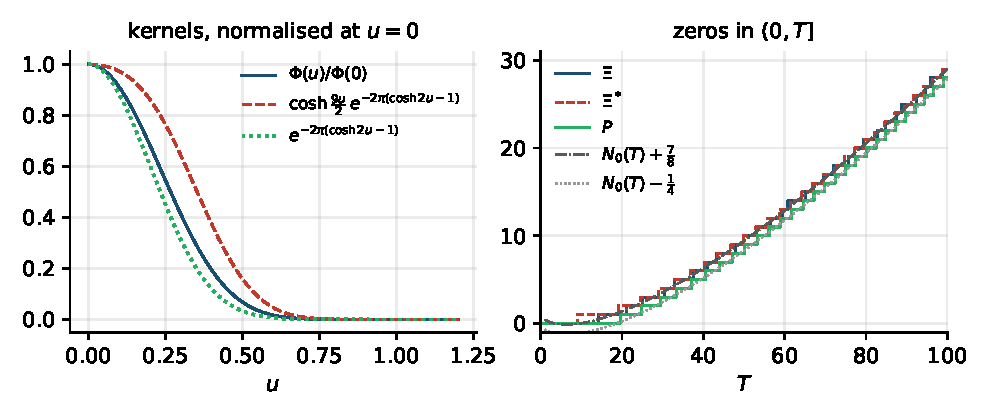
\includegraphics[width=\textwidth]{fig/biane_kernels.pdf}
\caption{Left: the kernel $\Phi$ of \eqref{eq:ch2:Phi}, P\'olya's asymptote $\Phi^*$ and the kernel $e^{-2\pi\cosh2u}$ of $P$, each divided by its value at $u=0$. Right: the zero counting functions of $\Xi$, $\Xi^*$ and $P$ on $(0,100]$, against $N_0(T)+\frac78$ and $N_0(T)-\frac14$, the mean values of the Riemann von Mangoldt formula and of Proposition~\ref{prop:biane:phase}, with $N_0(T)=\frac T{2\pi}\log\frac T{2\pi e}$. Drawn by \texttt{biane\_figs.py} from \texttt{biane\_polya.json}.}
\label{fig:biane:kernels}
\end{figure}

\begin{table}[htbp]
\centering\small
\begin{tabular}{rlll}
\toprule
$n$ & $\Xi$ & $\Xi^*$ & $P$\\
\midrule
1 & 14.135 & 8.993 & 19.538\\
2 & 21.022 & 19.065 & 24.897\\
3 & 25.011 & 24.475 & 29.370\\
4 & 30.425 & 28.975 & 33.383\\
5 & 32.935 & 33.007 & 37.099\\
6 & 37.586 & 36.737 & 40.600\\
7 & 40.919 & 40.249 & 43.936\\
8 & 43.327 & 43.595 & 47.140\\
9 & 48.005 & 46.807 & 50.234\\
10 & 49.774 & 49.908 & 53.236\\
11 & 52.970 & 52.916 & 56.158\\
12 & 56.446 & 55.843 & 59.009\\
13 & 59.347 & 58.700 & \\
\bottomrule
\end{tabular}
\qquad
\begin{tabular}{rrrrr}
\toprule
$T$ & $\Xi$ & $\Xi^*$ & $P$ & $N_0(T)$\\
\midrule
60 & 13 & 13 & 12 & 11.998\\
100 & 29 & 29 & 28 & 28.127\\
240 & 102 & 102 & 101 & 100.946\\
1000 & 649 & 649 & 647 & 647.741\\
\bottomrule
\end{tabular}
\caption{Left: the positive zeros below $60$ of $\Xi$, of P\'olya's $\Xi^*$ and of $P(\theta)=K_{i\theta/2}(2\pi)$. Right: the numbers of zeros in $(0,T]$ against $N_0(T)=\frac T{2\pi}\log\frac T{2\pi e}$. Computed by \texttt{biane\_polya.py}.}
\label{tab:biane:zeros}
\end{table}

The value $2\pi$ of the argument is forced. P\'olya's asymptotics for the zeros of $y\mapsto K_{iy}(2a)$, which Biane derives by stationary phase \cite[Section 3.5]{Biane09}, give $\frac T\pi\log\frac Ta-\frac T\pi+O(1)$ zeros with $0<y\le T$; for $P$ the zeros are at $\theta=2y$ with $a=\pi$, and the count in $(0,T]$ becomes $\frac T{2\pi}\log\frac T{2\pi}-\frac T{2\pi}+O(1)=N_0(T)+O(1)$. The constant $a=\pi$ comes from the factor $e^{-\pi e^{2u}}$ of the term $n=1$, and the $2$ in $\cosh2u$ turns $\frac T\pi\log\frac Ta$ into $\frac T{2\pi}\log\frac T{2\pi}$. Proposition~\ref{prop:biane:phase} gives the counting function of $P$ exactly.

Let $H^{(c)}_a$ be the first passage time of $B_t+ct$ to the level $a>0$, for a standard Brownian motion $B$ and a drift $c\ge0$, as in Appendix~\ref{app:notation}. Its density is $a(2\pi\tau^3)^{-1/2}e^{-(a-c\tau)^2/2\tau}$, the inverse Gaussian law of Table~\ref{tab:ch3:cat}, and its Laplace transform is $e^{a(c-\sqrt{c^2+2u})}$.

\begin{proposition}\label{prop:biane:mellin}
Let $H=H^{(c)}_a$ with $a=c=\sqrt{2\pi}$.
\begin{enumerate}
\item[(i)] $H$ has the density $\tau^{-3/2}e^{2\pi}e^{-\pi(\tau+1/\tau)}$ on $(0,\infty)$, and $1/H$ has the law of $H$ size biased by $H$.
\item[(ii)] $\E H^s=2e^{2\pi}K_{s-\frac12}(2\pi)$ for every $s\in\C$, so that $\E H^s=\E H^{1-s}$.
\item[(iii)] $P(\theta)=\frac12e^{-2\pi}\,\E H^{\frac12+\frac{i\theta}2}$ for every $\theta\in\C$.
\item[(iv)] $U=\frac12\log H$ has the density $2e^{2\pi}e^{-u}e^{-2\pi\cosh2u}$, and the law of $U$ size biased by $e^U$ has the density $e^{-2\pi\cosh2u}/K_0(2\pi)$, whose characteristic function is $P(\theta)/P(0)$.
\end{enumerate}
\end{proposition}

\begin{proof}
(i) With $a=c=\sqrt{2\pi}$, $(a-c\tau)^2/2\tau=\pi(\tau+1/\tau)-2\pi$ and $a/\sqrt{2\pi}=1$. The density of $1/H$ at $\sigma$ is $\sigma^{-2}$ times that of $H$ at $1/\sigma$, which is $\sigma^{-1/2}e^{2\pi}e^{-\pi(\sigma+1/\sigma)}$, that is $\sigma$ times the density of $H$ at $\sigma$; in particular $\E H=1$. (ii) The substitution $\tau=e^w$ and $K_\nu(x)=\int_0^\infty e^{-x\cosh w}\cosh(\nu w)\,dw$ \cite[(10.32.9)]{DLMF} give $\int_0^\infty\tau^{\nu-1}e^{-\pi(\tau+1/\tau)}\,d\tau=2K_\nu(2\pi)$, here with $\nu=s-\frac12$; the integral converges for every complex $\nu$, and $K_\nu=K_{-\nu}$ gives the symmetry. (iii) is (ii) at $s=\frac12+\frac{i\theta}2$. (iv) The substitution $\tau=e^{2u}$ turns the density of (i) into $2e^{2\pi}e^{-3u}e^{-2\pi\cosh2u}e^{2u}$; multiplying by $e^u$ and dividing by $\E H^{1/2}=2e^{2\pi}K_0(2\pi)$ gives the last density, and its characteristic function is $\int e^{-2\pi\cosh2u}e^{i\theta u}du/K_0(2\pi)=P(\theta)/P(0)$ by \eqref{eq:biane:P}.
\end{proof}

The parallel with $\Xi$ is exact. By the identity \eqref{bp:eq:bpy} of Biane, Pitman and Yor \cite{BPY01}, with $V=\frac\pi2S_2$, $2\xi(s)=\E V^{s/2}$, so $\Xi(\theta)=\frac12\E V^{\frac14+\frac{i\theta}2}$, and the kernel is $\Phi(u)=\frac12e^{u/2}f_Y(u)$ with $Y=\frac12\log V$: the P\'olya law of \eqref{eq:ch2:mgf} is the law of $Y$ size biased by $e^{Y/2}$, as the law of (iv) is that of $U$ size biased by $e^U$. On the critical line each function is the Fourier transform, in the logarithm of a hitting time, of the law tilted by a power of that time, and in both cases the evenness of the kernel is a reflection symmetry of the hitting time: $\tau\mapsto1/\tau$ for $H$, which is (i), and the functional equation $\E V^{s/2}=\E V^{(1-s)/2}$ for $V$, which comes from Jacobi's theta transformation. Numerically, \texttt{biane\_polya.py} integrates the density of (i) against $\tau^{\frac12+3.5i}$ and obtains $e^{-2\pi}\E H^{\frac12+3.5i}=7.261817522\times10^{-4}=2P(7)$, with an imaginary part of $2\times10^{-50}$, and it checks $\E S_2^s=2(2/\pi)^s\xi(2s)$, which is \eqref{bp:eq:bpy}, by integrating against the density of $S_2$ at $s=1$, $0.7$ and $\frac12+3i$ (values $0.6666666667$, $0.7384660825$ and $0.1205355309-0.3164244329i$, to ten digits both ways).

Both hitting times are GGCs, with the Thorin measures of Table~\ref{tab:ch3:cat}. For $H^{(c)}_a$ the Thorin measure is $a\,\{\pi\sqrt{2z-c^2}\}^{-1}\mathbf 1_{z>c^2/2}\,dz$, and the L\'evy density, $t^{-1}$ times its Laplace transform, is $a\,e^{-c^2t/2}(2\pi t^3)^{-1/2}$; at $a=c=1$ and $t=0.8$ both expressions give $0.3737294249$. For the Bessel hitting time, $\E e^{-uJ_a}=a\sqrt{2u}/\sinh(a\sqrt{2u})$ with $J_a\overset d=a^2J$, so $J_a+J'_a=a^2S_2$ has Thorin measure $2\sum_{n\ge1}\delta_{\pi^2n^2/2a^2}$ and L\'evy density $2t^{-1}\sum_ne^{-\pi^2n^2t/2a^2}$. The Thorin measure can also be read from the continuation of $\Psi(u)=-\log\E e^{-uX}$ across the cut: integrating the Stieltjes inversion \eqref{eq:ch3:inversion},
\[
U\big((0,z)\big)=\frac1\pi\im\Psi(-z+i0)\qquad(z>0\text{ not an atom}),
\]
because each factor $\log(1+u/w)$ with $w<z$ contributes $i\pi$ at $u=-z+i0$. For $H^{(c)}_a$, $\Psi(-z+i0)=a\big(i\sqrt{2z-c^2}-c\big)$ for $z>\frac{c^2}2$, so $U((0,z))=\frac a\pi\sqrt{2z-c^2}$, which is $0.7117625434$ at $a=c=1$, $z=3$, as the integral of the density gives; for $J_a+J'_a$, $\Psi(-\frac{\lambda^2}2+i0)=2\log\frac{\sin\lambda a}{\lambda a}$, which gains $2\pi i$ each time $\lambda a$ passes a multiple of $\pi$. Biane's dictionary identifies these Thorin measures with spectral measures. In his normalisation \cite[(2.1) to (2.3)]{Biane09} the generator $L_1=\frac12\frac{d^2}{dx^2}$ on $[0,\pi]$ with Dirichlet conditions has the eigenfunctions $\sin(kx)$, $k=1,2,\dots$, with eigenvalues $-\frac{k^2}2$, and the spectral measure $\sigma_1=\frac1\pi\sum_{n\ge1}\delta_{n^2/2}$; the generator $L_2=\frac12\frac{d^2}{dx^2}+\frac d{dx}$ on $[0,\infty)$ with a Dirichlet condition at $0$, selfadjoint in $L^2(e^{2x}dx)$, has the generalised eigenfunctions $e^{-x}\sin(kx)$, $k>0$, with eigenvalues $-\frac{k^2+1}2$, and the spectral measure $\sigma_2(d\lambda)=d\lambda/(\pi\sqrt{2\lambda-1})$ on $\lambda>\frac12$. In the wave number $k$ the two measures are $\frac1\pi$ times counting measure and $\frac1\pi$ times Lebesgue measure.

\begin{theorem}[Biane's dictionary, with corrected constants]\label{thm:biane:dict}
\begin{enumerate}
\item[(i)] The Thorin measure of $J_\pi+J'_\pi=\pi^2S_2$ is $2\pi\sigma_1$.
\item[(ii)] The Thorin measure of $H^{(1)}_1$ is $\sigma_2$.
\item[(iii)] The radial generator $\frac12\frac{d^2}{dx^2}+\cot x\frac d{dx}$ of Brownian motion on the unit sphere $S^3\cong SU(2)$ is the Doob transform of $L_1$ by its ground state $\sin x$, $\sin^{-1}(L_1+\frac12)\sin$, and the radial generator $\frac12\frac{d^2}{dx^2}+\coth x\frac d{dx}$ of Brownian motion on $\mathbb H^3=SL_2(\C)/SU(2)$ is the Doob transform of $L_2$ by the harmonic function $1-e^{-2x}$.
\end{enumerate}
\end{theorem}

\begin{proof}
(i) With $a=\pi$ the atoms $\pi^2n^2/2a^2$ are at $n^2/2$, with mass $2=2\pi\cdot\frac1\pi$. (ii) With $a=c=1$ the density $a\{\pi\sqrt{2z-c^2}\}^{-1}$ on $z>\frac{c^2}2$ is that of $\sigma_2$. (iii) For $f$ smooth, $\frac12(f\sin)''=\sin\cdot(\frac12f''+\cot x\,f'-\frac12f)$, so $\sin^{-1}(L_1+\frac12)(f\sin)=\frac12f''+\cot x\,f'$; and $L_2h=0$ for $h=1-e^{-2x}$, while $h^{-1}L_2(hf)=\frac12f''+(1+h'/h)f'$ with $1+h'/h=1+\frac{2e^{-2x}}{1-e^{-2x}}=\coth x$. The eigenfunctions are checked the same way: $L_2(e^{-x}s)=e^{-x}(\frac12s''-\frac12s)$.
\end{proof}

So Riemann's $\xi$ is attached to the compact group and to discrete spectrum, and P\'olya's $P$ to the hyperbolic space and to continuous spectrum. For P\'olya's function itself the parameters are $a=c=\sqrt{2\pi}$ rather than $a=c=1$; Brownian scaling gives $H^{(c)}_a\overset d=\frac ac\,H^{(\sqrt{ac})}_{\sqrt{ac}}$, so the level and the drift can always be made equal, which is the reciprocal symmetry of Proposition~\ref{prop:biane:mellin}(i), but their common value $\sqrt{ac}$ is $\sqrt{2\pi}$ for $P$ and $1$ in the dictionary. Part~(iii) corrects the direction of the Doob transforms in the note \cite{P26bia}, which has $L_1$ and $L_2$ as the transforms of the radial generators; Biane states them in the direction of (iii) \cite[Section 2.4]{Biane09}.

\begin{remark}[Constants in Biane's paper]\label{rem:biane:slips}
Readers of \cite{Biane09} next to this section should note the following. Biane's $K_\mu(x)=\int_0^\infty t^{\mu-1}e^{-\frac x2(t+t^{-1})}dt$ is twice the standard Macdonald function, and his kernel (3.1) is the $\Phi$ of \eqref{eq:ch2:Phi}; with that kernel $\Xi(z)=2\int_0^\infty\Phi(u)\cos(zu)\,du$ holds for the standard $\xi(s)=\frac12s(s-1)\pi^{-s/2}\Gamma(\frac s2)\zeta(s)$, so the factor $\frac12$ is missing from his displayed definition of $\xi$, and his Mellin formula $\E W_a^s=2(2a^2/\pi)^s\xi(2s)$ also uses the standard $\xi$ (both sides are $\frac23$ at $s=1$, $a=1$). In his Section 4.3 the L\'evy measure of $W_a=J_a+J'_a$ should be $2t^{-1}\sum_ne^{-\pi^2n^2t/2a^2}dt$, with the factor $t^{-1}$ and the $\frac12$ in the exponent, and that of the drifted first passage time should carry the level $x$ as a factor. His Thorin measure (4.1) should have its atoms at $\pi^2n^2/2a^2$, not at $n^2/a^2$; the density (4.2) should be $x\,dc/(\pi\sqrt{2c-a^2})$, which for $x=1$ is his density divided by $\sqrt2$, and the identity offered for it should read $(\pi t)^{-1/2}e^{-a^2t/2}=\int_{a^2/2}^\infty e^{-ct}\,dc/(\pi\sqrt{c-a^2/2})$, with $t$ in place of $t^3$. The measure (2.3) lives on $(\frac12,\infty)$, not on $[1,\infty)$. In Propositions 2.3 and 2.4 the drift and the harmonic function are oriented for the cone opposite to the one stated: with the cone $\{y_1\ge\dots\ge y_n\}$ the drift is $\rho'=(n-1,n-3,\dots,1-n)$ and the positive harmonic function is $\prod_{i<j}(1-e^{-2(y_i-y_j)})=e^{-\langle\rho',y\rangle}\prod_{i<j}2\sinh(y_i-y_j)$; the Vandermonde function $\prod_{i>j}(x_i-x_j)$ of his Proposition 2.1 is reversed in the same way, and is positive on the cone as $\prod_{i<j}(x_i-x_j)$. The eigenvalue of Proposition 2.6 is discussed in Remark~\ref{rem:biane:prop26}. With these corrections the dictionary of his Section 4.5 is the exact statement of Theorem~\ref{thm:biane:dict}.
\end{remark}

\subsection{The Wick rotation and the curvature family}\label{sec:biane:wick}

Biane closes his paper by observing that $\xi$ and P\'olya's function are related, through $SU(2)$ and $SL_2(\C)/SU(2)$, ``in this non obvious way'' \cite[Section 4.5]{Biane09}. The relation is a Wick rotation, the substitution of $iy$ for a real variable $y$ in a function analytic in $y$. In quantum mechanics a state evolves by the unitary group $e^{-itH}$, and Wick's device \cite{Wick54} rotates the time axis, $t=-i\tau$, which turns $e^{-itH}$ into the heat semigroup $e^{-\tau H}$; for $H=-\frac12\Delta+V$ the Feynman Kac formula $e^{-\tau H}f(x)=\E_x[\exp(-\int_0^\tau V(B_s)ds)f(B_\tau)]$ makes Brownian motion the Wick rotated form of quantum mechanics. The rotation keeps the spectrum, an eigenvalue $E$ appearing as a frequency $e^{-iEt}$ on one side and as a decay rate $e^{-E\tau}$ on the other, and it exchanges oscillation and positivity: probability laws, Laplace transforms and completely monotone functions live on the Euclidean side, Fourier transforms and their zeros on the real time side. A Thorin measure is spectral data that can be read on either side. The substitution $y\mapsto iy$ exchanges $\sinh$ and $\sin$, $\cosh$ and $\cos$, and Laplace and Fourier transforms, and through Cartan's duality between a symmetric space $G/K$ of noncompact type and its compact dual $U/K$ it reverses the sign of the curvature. Biane's paper contains the rotation in four places: in space (the sign of the curvature), in the Laplace variable, in time (heat kernels) and in the Mellin index. We take them in turn, after recalling the first part of his paper.

Let $H_n=\{y\in\R^n:\sum_iy_i=0\}$ and $\mathcal C=\{y\in H_n:y_1\ge\dots\ge y_n\}$. Biane describes three matrix valued Brownian motions of type A \cite[Section 2]{Biane09}. For traceless Hermitian Brownian motion the ordered eigenvalues perform Brownian motion in $\mathcal C$ conditioned in Doob's sense never to reach the boundary: the semigroup of Brownian motion killed at $\partial\mathcal C$ is the alternating sum $p^0_t(x,y)=\sum_{w\in S_n}\varepsilon(w)p_t(x,wy)$ (the reflection principle), the Vandermonde product $\prod_{i<j}(y_i-y_j)$ is its positive harmonic function vanishing on $\partial\mathcal C$, and the Doob transform is Dyson's Brownian motion \cite{Dyson62}. For Brownian motion $g_t$ on $SL_n(\C)$, the logarithms of the singular values, the radial part of Brownian motion on $SL_n(\C)/SU(n)$, perform Brownian motion in $\mathcal C$ with generator $\frac12\Delta+\langle\nabla\log\tilde h,\nabla\rangle$, $\tilde h(y)=\prod_{i<j}\sinh(y_i-y_j)$ \cite{JonesOConnell06}, which is Brownian motion with drift $\rho'=(n-1,n-3,\dots,1-n)$, killed at $\partial\mathcal C$, transformed by the harmonic function of Remark~\ref{rem:biane:slips}; here the Martin boundary is large, with a point for each direction in the cone. For Brownian motion on $SU(n)$ the eigenvalues $e^{i\theta_j}$, with $\sum_j\theta_j=0$, live in the alcove $\theta_1\ge\dots\ge\theta_n$, $\theta_1-\theta_n\le2\pi$, a fundamental domain of the affine Weyl group $S_n\ltimes((2\pi\mathbb Z)^n\cap H_n)$; the killed semigroup is the alternating sum over that group, and the eigenvalue process is the Doob transform by the Dirichlet ground state $\prod_{j>k}(e^{i\theta_j}-e^{i\theta_k})$, which is a constant multiple of $\prod_{j<k}\sin\frac{\theta_j-\theta_k}2$ because $\sum_j\theta_j=0$.

The three Doob functions are one function at three values of a curvature parameter. For real $\kappa$ put $s_\kappa(z)=\sin(\sqrt\kappa z)/\sqrt\kappa$, so that $s_{-1}=\sinh$, $s_0(z)=z$ and $s_1=\sin$, and
\[
h_\kappa(y)=\prod_{i<j}s_\kappa(y_i-y_j),\qquad|\rho|^2=\sum_{j=1}^n(n+1-2j)^2=\frac{n(n^2-1)}3 .
\]

\begin{proposition}\label{prop:biane:curv}
For every real $\kappa$ and every $n\ge2$, $\Delta h_\kappa=-\kappa|\rho|^2h_\kappa$ on $H_n$.
\end{proposition}

\begin{proof}
For $\kappa=-1$, write $\prod_{i<j}2\sinh(y_i-y_j)=\prod_{i<j}e^{-(y_i+y_j)}(e^{2y_i}-e^{2y_j})$. The Vandermonde determinant gives $\prod_{i<j}(e^{2y_i}-e^{2y_j})=\det(e^{2(n-j)y_i})$, and on $H_n$ the factor $\prod_{i<j}e^{-(y_i+y_j)}=e^{-(n-1)\sum_iy_i}$ is one, so the exponents $2(n-j)$ may be replaced by $2(n-j)-(n-1)=n+1-2j$: $\prod_{i<j}2\sinh(y_i-y_j)=\sum_{w\in S_n}\varepsilon(w)e^{\langle w\rho',y\rangle}$, the Weyl denominator formula. Each $w\rho'$ lies in $H_n$ and has $|w\rho'|^2=|\rho|^2$, so each exponential is an eigenfunction of the Laplacian of $H_n$ with eigenvalue $|\rho|^2$, and $\Delta h_{-1}=|\rho|^2h_{-1}$. This identity between entire functions of $y\in H_n\otimes\C$ continues analytically. For $\kappa<0$, $h_\kappa(y)$ is a constant times $h_{-1}(\sqrt{-\kappa}\,y)$, and the scaling multiplies the Laplacian by $-\kappa$; for $\kappa>0$, $s_\kappa(z)=\sinh(i\sqrt\kappa z)/(i\sqrt\kappa)$, so $h_\kappa(y)$ is a constant times $h_{-1}(i\sqrt\kappa\,y)$, and the substitution multiplies the Laplacian by $(i\sqrt\kappa)^2=-\kappa$. At $\kappa=0$, $h_0$ is the Vandermonde product, the limit of $h_\kappa$ as $\kappa\to0$, since $s_\kappa(z)=z-\kappa z^3/6+O(\kappa^2)$, and it is harmonic.
\end{proof}

\texttt{biane\_polya.py} checks the proposition with a symbolic Laplacian at random points of $H_n$ for $n=2,3,4$ and $\kappa=-1,0,1$, where $|\rho|^2=2$, $8$, $20$. So Biane's three semigroups are one formula,
\[
q^{(\kappa)}_t(x,y)=\frac{h_\kappa(y)}{h_\kappa(x)}\,e^{\kappa|\rho|^2t/2}\,p^{0}_t(x,y),\qquad\kappa\in\{-1,0,1\},
\]
with generator $\frac12\Delta+\langle\nabla\log h_\kappa,\nabla\rangle$, where $p^0$ is the killed kernel of the chamber $\mathcal C$ for $\kappa\le0$ and of the alcove $\{y_1\ge\dots\ge y_n,\ y_1-y_n\le\pi\}$ for $\kappa=1$; for $\kappa=1$ the coordinates are the half angles $y=\theta/2$, in which $h_1$ is the positive Dirichlet ground state of the alcove. The rotation $y\mapsto iy$ sends $h_\kappa$ to a constant times $h_{-\kappa}$, since $s_\kappa(iz)=is_{-\kappa}(z)$: it exchanges the noncompact and the compact Doob functions, passes through Dyson's Brownian motion at the flat point $\kappa=0$, and reverses the sign of the ground energy, $\frac12\Delta h_\kappa=-\frac\kappa2|\rho|^2h_\kappa$, which is $+\frac12|\rho|^2$ for $SL_n(\C)/SU(n)$ and $-\frac12|\rho|^2=\frac{n-n^3}6$ for $SU(n)$ in the half angles.

\begin{remark}[The eigenvalue of Biane's Proposition 2.6]\label{rem:biane:prop26}
Biane endows the Lie algebra of $SU(n)$ with the form $\langle A,B\rangle=-\operatorname{Tr}(AB)$, in which the angles $\theta_j$ perform standard Brownian motion in $H_n$, and states that the ground state $\prod_{j<k}\sin\frac{\theta_j-\theta_k}2$ has the eigenvalue $\frac{n-n^3}6$ for $\frac12\Delta$ \cite[Proposition 2.6]{Biane09}. By Proposition~\ref{prop:biane:curv} in the half angles, the eigenvalue for $\frac12\Delta_\theta$ is $\frac14\cdot\frac{n-n^3}6=\frac{n-n^3}{24}$; more generally, for the form $-c\operatorname{Tr}(AB)$ it is $\frac{n-n^3}{24c}$. Biane's value holds for $c=\frac14$, that is when the half angles are standard Brownian motion. His rank one discussion uses a third normalisation, $c=\frac12$, in which $SU(2)$ is the unit sphere $S^3$, the angle $x\in[0,\pi]$ has the generator $\frac12\frac{d^2}{dx^2}+\cot x\frac d{dx}$ of Theorem~\ref{thm:biane:dict}(iii), and the ground energy is $\frac{2-8}{12}=-\frac12$. \texttt{biane\_polya.py} confirms $\frac12\Delta_\theta h/h=-\frac14,-1,-\frac52$ for $n=2,3,4$.
\end{remark}

In rank one the curvature family is the radial part of Brownian motion on the three dimensional space form of curvature $\kappa$, with generator $\frac12\frac{d^2}{dx^2}+\sqrt\kappa\cot(\sqrt\kappa x)\frac d{dx}$: the sphere of radius $\kappa^{-1/2}$ for $\kappa>0$, the Bessel process of dimension three for $\kappa=0$, and the hyperbolic space of curvature $\kappa$ for $\kappa<0$. Let $J^{(\kappa)}_a$ be its hitting time of the radius $a$ from the centre, with $a<\pi/\sqrt\kappa$ when $\kappa>0$; then $J^{(0)}_a=J_a$, whose Laplace transform is classical \cite{CiesielskiTaylor62}. For $\kappa<0$ the generator is that of the Bessel process of dimension three with drift $\sqrt{-\kappa}$ \cite[(2.5)]{SalminenVallois07}, the norm of a three dimensional Brownian motion with drift of that length, and the case $\kappa<0$ of the next proposition also follows from the Cameron Martin formula, since for Brownian motion without drift started at the centre the exit place of a ball is uniform and independent of the exit time.

\begin{proposition}\label{prop:biane:skappa}
For $u\ge0$,
\[
\E e^{-uJ^{(\kappa)}_a}=\frac{\sqrt{2u-\kappa}\;s_\kappa(a)}{\sinh\big(a\sqrt{2u-\kappa}\big)},
\]
the Laplace transform of a GGC with Thorin measure $\sum_{n\ge1}\delta_{\pi^2n^2/2a^2-\kappa/2}$. Equivalently, the law of $J^{(\kappa)}_a$ is the exponential tilt $e^{\kappa t/2}\,\Pr(J_a\in dt)/\E e^{\kappa J_a/2}$ of the law of $J_a$.
\end{proposition}

\begin{proof}
The generator is the Doob transform of $\frac12\frac{d^2}{dx^2}$ by $s=s_\kappa$, since $s''=-\kappa s$ gives $s^{-1}(\frac12\frac{d^2}{dx^2}+\frac\kappa2)(sf)=\frac12f''+\frac{s'}sf'$ and $s'/s=\sqrt\kappa\cot(\sqrt\kappa x)$. Hence $f(x)=\sinh(x\sqrt{2u-\kappa})/s_\kappa(x)$ satisfies $\frac12f''+\frac{s'}sf'=s^{-1}(\frac12g''+\frac\kappa2g)=uf$ with $g=\sinh(x\sqrt{2u-\kappa})$, and $f$ is, up to a constant factor, the positive increasing solution that stays bounded at $0$, with $f(0+)=\sqrt{2u-\kappa}$. Hence $\E_xe^{-uJ^{(\kappa)}_a}=f(x)/f(a)$ for $0<x<a$, and letting $x\downarrow0$ gives $\E e^{-uJ^{(\kappa)}_a}=f(0+)/f(a)$, which is the formula; for $\kappa>2u$ the square roots are imaginary and the formula is read through $\sinh(ix)/i=\sin x$. As a function of $u$ the denominator divided by $\sqrt{2u-\kappa}$ is entire of order $\frac12$, with zeros where $a\sqrt{2u-\kappa}=i\pi n$, that is at $u=-(\pi^2n^2/2a^2-\kappa/2)$, all negative under the hypothesis on $a$; Hadamard's product in genus zero gives the Thorin measure. The tilt is the formula at $u-\frac\kappa2$ for $\kappa=0$, divided by its value at $u=0$, since $\sqrt{-\kappa}/\sinh(a\sqrt{-\kappa})=1/s_\kappa(a)$.
\end{proof}

At $u=0.7$, $a=0.9$ and $\kappa=1,-1,\frac13$, \texttt{biane\_polya.py} obtains $0.82508145967889$, $0.84051739205883$ and $0.83070660638487$, each the same from the formula, from the tilt and from the product over the Thorin atoms, and the residual of the differential equation is below $10^{-40}$. Three consequences clarify the dictionary. First, Riemann's clock $J_a+J'_a$ is the flat member $\kappa=0$, and its link with $SU(2)$ in Theorem~\ref{thm:biane:dict} is spectral rather than geometric: the atoms $\pi^2n^2/2a^2$ are the Dirichlet spectrum of $\frac12\frac{d^2}{dx^2}$ on $[0,a]$, which for $a=\pi$ is the spectrum of the radial generator of $SU(2)$ shifted by its ground energy $\frac12$. Second, the hyperbolic member $\kappa=-1$ has the discrete atoms $\pi^2n^2/2a^2+\frac12$; P\'olya's continuous measure comes instead from a first passage over a level on the half line, a Dirichlet problem on $[0,\infty)$ with continuous spectrum. Third, the tilt destroys the reciprocal symmetry of $J_a+J'_a$ that encodes the functional equation. With $W=J^{(\kappa)}_1+J'^{(\kappa)}_1$, the function $(\frac\pi2)^s\E W^s$ equals $2\xi(2s)$ for $\kappa=0$ and is symmetric under $s\mapsto\frac12-s$: it takes the value $0.9963110325$ at both $s=0.1$ and $s=0.4$. For $\kappa=1$ the two values are $1.002917197$ and $1.023703077$. A curvature interpolation between the two clocks must therefore be sought in a class that keeps the symmetry (Question~\ref{q:biane:curv}).

Replacing $u$ by a negative value in $\E e^{-uX}$ continues the transform across the origin, and this is the rotation of the Laplace variable used in the inversion formula above. For the curvature family the reciprocal of the transform becomes, for $u<\frac\kappa2$, the damped sine $\sin(a\sqrt{\kappa-2u})/(\sqrt{\kappa-2u}\,s_\kappa(a))$, whose zeros sit at minus the Thorin atoms and slide with $\kappa$; for the drifted clock the reciprocal $e^{a(\sqrt{c^2+2u}-c)}$ becomes $e^{-ac}e^{ia\sqrt{2|u|-c^2}}$ beyond the branch point $u=-\frac{c^2}2$, which has constant modulus and no zeros. Poles of the transform, which require discrete spectrum, here that of a compact space, give atoms of the Thorin measure; a branch cut gives a density. Figure~\ref{fig:biane:wick} shows both.

\begin{figure}[htbp]
\centering
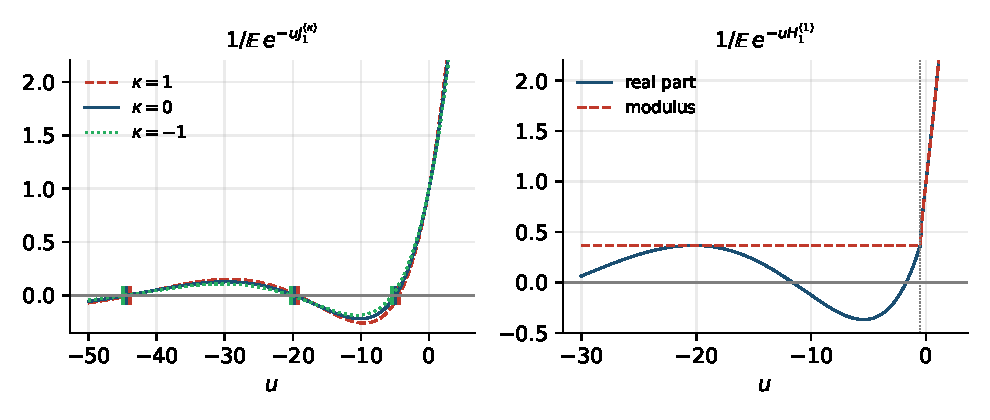
\includegraphics[width=\textwidth]{fig/biane_wick.pdf}
\caption{The Wick rotation of the Laplace variable. Left: $1/\E e^{-uJ^{(\kappa)}_1}$ for $\kappa=1,0,-1$, positive and increasing for $u>0$ and a damped sine for $u<\frac\kappa2$, vanishing at minus the Thorin atoms $\pi^2n^2/2-\kappa/2$ (marks). Right: $1/\E e^{-uH^{(1)}_1}=e^{\sqrt{1+2u}-1}$, real part and modulus; beyond the branch point $u=-\frac12$ (dotted) the modulus is constant, $e^{-1}$, and there are no zeros, the signature of a Thorin density. Drawn by \texttt{biane\_figs.py}.}
\label{fig:biane:wick}
\end{figure}

The rotation of time relates the heat kernels of the two dual spaces. Writing $x=-iy$ gives $\frac d{dx}=i\frac d{dy}$ and $\coth(-iy)=i\cot y$, so $\frac12\frac{d^2}{dx^2}+\coth x\frac d{dx}$ becomes $-(\frac12\frac{d^2}{dy^2}+\cot y\frac d{dy})$, and the Doob functions $\sinh$ and $\sin$ are exchanged. The radial heat kernels of $\frac12\Delta$, relative to the Riemannian volume, are
\begin{gather*}
p^{\mathbb H^3}_t(r)=\frac{e^{-t/2}}{(2\pi t)^{3/2}}\,\frac r{\sinh r}\,e^{-r^2/2t},\\
p^{S^3}_t(\omega)=\frac{e^{t/2}}{(2\pi t)^{3/2}}\sum_{k\in\mathbb Z}\frac{\omega+2\pi k}{\sin\omega}\,e^{-(\omega+2\pi k)^2/2t},
\end{gather*}
and the term $k=0$ of the second is, up to the constant factor $(-1)^{-3/2}$, the first after $r\mapsto i\omega$, $t\mapsto-t$, a genuine Wick rotation of time; the sum over $k$ is the method of images over the affine Weyl group, which makes the kernel periodic. \texttt{biane\_polya.py} checks that both kernels integrate to one against $4\pi\sinh^2r\,dr$ and $4\pi\sin^2\omega\,d\omega$ at $t=0.3$ and $t=1$. In rank $n$ the same statement is the formula for $q^{(\kappa)}_t$, whose factor $e^{\kappa|\rho|^2t/2}$ changes sign with $\kappa$ as $e^{\mp t/2}$ does here. Compactness replaces the continuous spectrum $[\frac12,\infty)$ of $-L_2$ by the lattice $\{\frac{n^2}2\}$ of $-L_1$, which is the passage from $\sigma_2$ to $\sigma_1$ in Theorem~\ref{thm:biane:dict}.

The fourth rotation acts on the Mellin index. The substitution $s=\frac12+i\theta$ turns real Mellin moments into Fourier transforms of a tilted law, and Biane's contour shift $w\mapsto w+\frac{i\pi}2$ \cite[Section 3.5]{Biane09}, with $\cosh(w+\frac{i\pi}2)=i\sinh w$, turns the damped integrand $e^{zw-2a\cosh w}$ into an oscillating one on which stationary phase locates the zeros. For $P$ this is the map $\mu\mapsto i\mu$ on the index of $K_\mu$, and Section~\ref{sec:biane:kg} shows that the index is the eigenvalue of a boost, which the rotation turns into an angular momentum. Table~\ref{tab:biane:wick} collects the dictionary. Atoms of a Thorin measure on the Euclidean side become poles after the rotation, and poles require discrete spectrum, which for these radial Brownian motions, with no potential, means a compact space. That is why $\xi$, whose time side Thorin measure is atomic, is attached to $SU(2)$, while $P$, whose time side measure has a density, is attached to $\mathbb H^3$.

\begin{table}[htbp]
\centering\small
\begin{tabular}{@{}p{0.27\textwidth}p{0.33\textwidth}p{0.33\textwidth}@{}}
\toprule
 & real time side & Euclidean side\\
\midrule
evolution & $e^{-itH}$, oscillating & $e^{-\tau H}$, positive\\
geometry & compact, $S^3=SU(2)$, $\kappa=1$ & noncompact, $\mathbb H^3$, $\kappa=-1$\\
Doob function & $\prod\sin$ & $\prod\sinh$\\
ground energy of $\frac12\Delta$ & $-\frac12|\rho|^2$ & $+\frac12|\rho|^2$\\
radial spectrum & discrete, $\{\frac{n^2}2\}$ & continuous, $[\frac12,\infty)$\\
transform & Fourier, $\E e^{i\lambda X}$ & Laplace, $\E e^{-uX}$\\
Thorin measure & poles and cuts & a positive measure\\
Bessel function & $K_{i\nu}$, oscillating, with zeros & $K_\nu$, positive\\
symmetry of Section~\ref{sec:biane:kg} & boost, rapidity & rotation, angle\\
zeros of $\Xi$ and $P$ & live here & are Thorin atoms here\\
\bottomrule
\end{tabular}
\caption{The two sides of the Wick rotation.}
\label{tab:biane:wick}
\end{table}

\subsection{The zeros of \texorpdfstring{$P$}{P} as a Dirichlet spectrum}\label{sec:biane:zeros}

Put $\psi_\mu(x)=K_\mu(e^x)$. Since $\frac d{dx}=r\frac d{dr}$ for $r=e^x$, the modified Bessel equation $r^2K''+rK'-(r^2+\mu^2)K=0$ becomes
\[
-\psi_\mu''+e^{2x}\psi_\mu=-\mu^2\psi_\mu ,
\]
a Schr\"odinger equation with the Liouville potential $e^{2x}$, in which the index enters only through the energy $-\mu^2$. Let $x_0=\log2\pi$, and let $A_P=-\frac{d^2}{dx^2}+e^{2x}$ act in $L^2([x_0,\infty))$ with a Dirichlet condition at $x_0$. Biane recalls this spectral interpretation of the zeros of the Macdonald function as well known, with Titchmarsh's treatise on eigenfunction expansions \cite{TitchmarshEigen46} as its reference, and notes that P\'olya does not mention it \cite[Section 3.3]{Biane09}. We write $\nu_1<\nu_2<\cdots$ for the positive zeros of $\nu\mapsto K_{i\nu}(2\pi)$, so that $P$ vanishes at $\theta=\pm2\nu_n$.

\begin{proposition}\label{prop:biane:liouville}
\begin{enumerate}
\item[(i)] $A_P$ is selfadjoint, has compact resolvent, and $A_P\ge4\pi^2$.
\item[(ii)] A number $\lambda$ is an eigenvalue of $A_P$ if and only if $\lambda=\nu^2$ with $\nu>0$ and $K_{i\nu}(2\pi)=0$, and the eigenfunction is then $K_{i\nu}(e^x)$. In particular every zero of $P$ is real, of absolute value at least $4\pi$, and the zeros of $P$ are the numbers $\pm2\nu_n$ with $\nu_n^2$ running over the spectrum of $A_P$.
\item[(iii)] Every eigenvalue of $A_P$ is simple, and every zero of $\mu\mapsto K_\mu(2\pi)$ and of $P$ is simple. More precisely, for $\nu>0$ and every $y\in\R$,
\begin{equation}\label{eq:biane:wronski}
\psi_{i\nu}'(y)\,\partial_\nu\psi_{i\nu}(y)-\psi_{i\nu}(y)\,\partial_\nu\psi_{i\nu}'(y)=-2\nu\int_y^\infty\psi_{i\nu}(x)^2\,dx<0 .
\end{equation}
\end{enumerate}
\end{proposition}

\begin{proof}
(i) The endpoint $x_0$ is regular, and the potential is bounded below, so the equation is in the limit point case at $+\infty$ and the Dirichlet realisation is selfadjoint; since $e^{2x}\to\infty$, the resolvent is compact. For $f$ in the form domain, $\langle A_Pf,f\rangle=\int_{x_0}^\infty(|f'|^2+e^{2x}|f|^2)\,dx\ge e^{2x_0}\|f\|^2=4\pi^2\|f\|^2$. (ii) For every complex $\mu$, $K_\mu(r)=\sqrt{\pi/2r}\,e^{-r}(1+O(1/r))$ as $r\to\infty$ \cite[(10.40.2)]{DLMF}, so $\psi_\mu$ is a nonzero solution in $L^2$ near $+\infty$, and in the limit point case it is the only one up to a constant factor. Hence $-\mu^2$ is an eigenvalue exactly when $\psi_\mu(x_0)=K_\mu(2\pi)=0$. By (i) such an eigenvalue is real and at least $4\pi^2$, so $\mu=\pm i\nu$ with $\nu\ge2\pi$; since $P(\theta)=K_{i\theta/2}(2\pi)$, the zeros of $P$ are $\theta=\pm2\nu$. (iii) Two eigenfunctions with the same eigenvalue both vanish at $x_0$, so they are proportional. For \eqref{eq:biane:wronski}, put $\phi=\partial_\nu\psi_{i\nu}$; differentiating $\psi_{i\nu}''=(e^{2x}-\nu^2)\psi_{i\nu}$ in $\nu$ gives $\phi''=(e^{2x}-\nu^2)\phi-2\nu\psi_{i\nu}$, so that $(\psi_{i\nu}'\phi-\psi_{i\nu}\phi')'=2\nu\psi_{i\nu}^2$. Both functions and their derivatives decay like $\exp(-e^x)$, and integrating from $y$ to $\infty$ gives the identity. The function $\psi_{i\nu}$ is real valued and not identically zero, so the right side is negative. At $y=x_0$ and $\nu=\nu_n$ the second term on the left vanishes, so $\partial_\nu K_{i\nu}(2\pi)\ne0$ at $\nu_n$, which is the simplicity of the zero.
\end{proof}

The proposition is P\'olya's theorem that $P$ has only real zeros, obtained from selfadjointness, and $A_P$ is an explicit Hilbert P\'olya operator for $P$. Biane also writes the equation in Dirac form \cite[Section 3.4]{Biane09}. With $D=\frac d{dx}$ and $\mathcal A=D+\frac12+e^x$, whose formal adjoint is $\mathcal A^\dagger=-D+\frac12+e^x$, the system $\mathcal Af=\gamma g$, $\mathcal A^\dagger g=\gamma f$ gives $\mathcal A^\dagger\mathcal Af=\gamma^2f$, and a direct computation gives $\mathcal A^\dagger\mathcal A=A_P+\frac14$. With the Dirichlet condition on $f$ the Dirac eigenvalues are therefore $\gamma=\pm(\nu_n^2+\frac14)^{1/2}$, not $\pm\nu_n$; the shift $\frac14$, which Biane writes as $\gamma^2-\frac14$, is missing from the note \cite{P26bia}. In the variable $u=e^x$ the system reads $(u\frac d{du}+\frac12+u)f=\gamma g$, $(-u\frac d{du}+\frac12+u)g=\gamma f$, and since $u\frac d{du}+\frac12$ is $i$ times the symmetrised dilation operator $\frac12(up+pu)$, $p=-i\frac d{du}$, it is the Hamiltonian $xp$ of Berry and Keating \cite{BerryKeating99} perturbed by the potential $u$, as Biane remarks.

The zeros of $P$ obey an exact quantisation rule. Let $I_\mu$ be the modified Bessel function of the first kind, and for real $\nu$ put
\begin{equation}\label{eq:biane:phase}
\vartheta_P(\nu)=\im\log\Gamma(1+i\nu)-\nu\log\pi-\arg{}_0F_1(;1+i\nu;\pi^2),
\end{equation}
with the branches continuous in $\nu$ and equal to zero at $\nu=0$, where ${}_0F_1(;1;\pi^2)=I_0(2\pi)>0$. Write $N_P(T)$ for the number of zeros of $P$ in $(0,T]$ and
\[
x(T)=\frac1\pi\vartheta_P\big(\tfrac T2\big),\qquad N_0(T)=\frac T{2\pi}\log\frac T{2\pi e}.
\]

\begin{proposition}\label{prop:biane:phase}
\begin{enumerate}
\item[(i)] For $\nu>0$, $I_{i\nu}(2\pi)\ne0$ and
\[
K_{i\nu}(2\pi)=\frac{\pi\,|I_{i\nu}(2\pi)|\,\sin\vartheta_P(\nu)}{\sinh\pi\nu}.
\]
\item[(ii)] $\vartheta_P(\nu)>0$ for $\nu>0$, $\vartheta_P(\nu_n)=n\pi$ for every $n$, and the number of zeros of $\nu\mapsto K_{i\nu}(2\pi)$ in $(0,\nu)$ is $\lceil\vartheta_P(\nu)/\pi\rceil-1$. Equivalently, $N_P(T)=\lfloor x(T)\rfloor$ for every $T>0$ that is not a zero of $P$.
\item[(iii)] As $\nu\to\infty$,
\[
\vartheta_P(\nu)=\nu\log\frac\nu\pi-\nu+\frac\pi4+\frac{\pi^2-\frac1{12}}\nu+O(\nu^{-3}),
\]
so that $x(T)=N_0(T)+\frac14+\big(2\pi-\frac1{6\pi}\big)\frac1T+O(T^{-3})$ as $T\to\infty$.
\end{enumerate}
\end{proposition}

\begin{proof}
(i) For real $r>0$, $I_{-i\nu}(r)=\overline{I_{i\nu}(r)}$, and $K_\mu=\pi(I_{-\mu}-I_\mu)/(2\sin\mu\pi)$ gives $K_{i\nu}(r)=-\pi\im I_{i\nu}(r)/\sinh\pi\nu$. The series $I_{i\nu}(r)=(r/2)^{i\nu}\,{}_0F_1(;1+i\nu;r^2/4)/\Gamma(1+i\nu)$ shows that, for $r>0$,
\[
\vartheta(\nu,r)=\im\log\Gamma(1+i\nu)-\nu\log\frac r2-\arg{}_0F_1\big(;1+i\nu;\tfrac{r^2}4\big)
\]
satisfies $I_{i\nu}(r)=|I_{i\nu}(r)|e^{-i\vartheta(\nu,r)}$, and $\vartheta_P(\nu)=\vartheta(\nu,2\pi)$; this gives the formula. If $I_{i\nu}(r)$ vanished, so would $I_{-i\nu}(r)$, against the Wronskian $I_\mu I_{-\mu}'-I_\mu'I_{-\mu}=-2\sin(\mu\pi)/(\pi r)$ \cite[(10.28.1)]{DLMF}, which is not zero for $\mu=i\nu$. So ${}_0F_1$ does not vanish on $[0,\infty)\times(0,\infty)$, and $\vartheta$ is defined there as a continuous function with $\vartheta(0,r)=0$. (ii) The same Wronskian, written for $I=I_{i\nu}$ and $\bar I=I_{-i\nu}$, gives $\im(I'/I)=\sinh(\pi\nu)/(\pi r|I|^2)$, hence $\partial_r\vartheta(\nu,r)=-\sinh(\pi\nu)/(\pi r|I_{i\nu}(r)|^2)<0$. As $r\to\infty$, $I_{i\nu}(r)\sim e^r/\sqrt{2\pi r}$ and $K_{i\nu}(r)\sim\sqrt{\pi/2r}\,e^{-r}$ uniformly for $\nu$ in compact sets, so $\sin\vartheta(\nu,r)=\sinh(\pi\nu)K_{i\nu}(r)/(\pi|I_{i\nu}(r)|)\to0$ and $\cos\vartheta(\nu,r)>0$ for large $r$; by continuity in $\nu$ from $\nu=0$, $\vartheta(\nu,r)\to0$. So for fixed $\nu>0$ the function $r\mapsto\vartheta(\nu,r)$ decreases from $\vartheta_P(\nu)$ at $r=2\pi$ to $0$ at $r=\infty$; in particular $\vartheta_P(\nu)>0$, and $r\mapsto K_{i\nu}(r)$ has exactly $\lceil\vartheta_P(\nu)/\pi\rceil-1$ zeros in $(2\pi,\infty)$, one at each crossing of a multiple of $\pi$. On the other hand, by \eqref{eq:biane:wronski} at a zero $y$ of $\psi_{i\nu}$, $\psi_{i\nu}'(y)\,\partial_\nu\psi_{i\nu}(y)<0$, so every zero of $x\mapsto K_{i\nu}(e^x)$ moves to the right as $\nu$ increases; no zero comes in from $+\infty$, where $K_{i\nu}(r)>0$ uniformly for $\nu$ in compact sets, and zeros cannot appear in pairs, since they are simple. So the number of zeros in $(x_0,\infty)$ is zero for small $\nu$ and increases by one exactly when $\nu$ passes some $\nu_n$, where a zero enters through $x_0$: it equals the number of $\nu_n<\nu$. Comparing the two counts gives the statement, and $\vartheta_P(\nu_n)\in\pi\mathbb Z$ with the count passing from $n-1$ to $n$ gives $\vartheta_P(\nu_n)=n\pi$. (iii) Stirling's series gives $\im\log\Gamma(1+i\nu)=\nu\log\nu-\nu+\frac\pi4-\frac1{12\nu}+O(\nu^{-3})$, and with $b=1+i\nu$, $\log{}_0F_1(;b;z)=z/b-z^2/(2b^2(b+1))+O(b^{-3})$, so $\arg{}_0F_1(;1+i\nu;\pi^2)=\im\frac{\pi^2}{1+i\nu}+O(\nu^{-3})=-\frac{\pi^2}\nu+O(\nu^{-3})$. With $\nu=T/2$, $\frac1\pi(\nu\log\frac\nu\pi-\nu)=N_0(T)$.
\end{proof}

So the zeros of $P$ are the solutions of $\vartheta_P(\nu_n)=n\pi$, and their counting function is the floor of a smooth function, with no fluctuating remainder. Writing $s_P(T)=\{x(T)\}-\frac12$ for the sawtooth,
\[
N_P(T)=N_0(T)-\frac14-s_P(T)+\Big(2\pi-\frac1{6\pi}\Big)\frac1T+O(T^{-3}),
\]
against the Riemann von Mangoldt formula $N(T)=\vartheta(T)/\pi+1+S(T)$ of Section~\ref{ch:classical}, which with $\vartheta(T)=\frac T2\log\frac T{2\pi}-\frac T2-\frac\pi8+\frac1{48T}+O(T^{-3})$ reads
\[
N(T)=N_0(T)+\frac78+S(T)+\frac1{48\pi T}+O(T^{-3}).
\]
The two counting functions share the main term $N_0$, but their mean constant terms differ by $\frac78+\frac14=\frac98$, and the fluctuation of $N_P$ is the bounded sawtooth of a quantisation rule where that of $N$ is $S(T)$. These two facts govern the comparison of the two Poisson traces in Section~\ref{sec:biane:cm}. Table~\ref{tab:biane:zeros} shows the effect: $N(1000)-N_P(1000)=2$, with $N_0(1000)=647.741$. The note \cite{P26bia} states that the semiclassical count of $A_P$ is exactly the main term of the Riemann von Mangoldt formula. The count is
\[
N_{\rm WKB}(\nu)=\frac1\pi\int_{x_0}^{\log\nu}\sqrt{\nu^2-e^{2x}}\,dx=\frac1\pi\Big(\nu\operatorname{arccosh}\frac\nu{2\pi}-\sqrt{\nu^2-4\pi^2}\Big),
\]
and its expansion gives $N_{\rm WKB}(T/2)=N_0(T)+\frac{2\pi}T+O(T^{-3})$: it agrees with the main term up to $2\pi/T$, not exactly. Its phase $\varphi(\nu)=\pi N_{\rm WKB}(\nu)+\frac\pi4$ is the phase of Debye's expansion of $K_{i\nu}(2\pi)$ for large $\nu$, the term $\frac\pi4$ being the Maslov correction at the turning point, and by (iii) $\vartheta_P(\nu)-\varphi(\nu)=-\frac1{12\nu}+O(\nu^{-3})$.

\texttt{biane\_polya.py} computes $\vartheta_P$ from \eqref{eq:biane:phase} with mpmath at $40$ digits \cite{mpmath} and solves $\vartheta_P(\nu)=n\pi$ by the secant method for every $\nu_n\le1000$, $1516$ zeros. It checks (i) against Arb's $K_{i\nu}(2\pi)$ \cite{Arb} at $\nu=0.5$, $3$, $9.5$, $25$, $101.3$ and $700$, with relative differences below $4\times10^{-37}$, encloses the first $40$ zeros to $10^{-25}$ by sign changes of Arb balls, and finds $137$ sign changes of $K_{i\nu}(2\pi)$ on a grid of step $0.02$ in $(0,150]$, the number of $\nu_n$ below $150$. The first zeros are
\begin{gather*}
\nu_1=9.768770083509978,\qquad\nu_2=12.44848789277578,\\
\nu_3=14.68495977595033,\qquad\nu_4=16.69157893829242,
\end{gather*}
and $\nu_1$ agrees with the first zero of $K_{i\theta}(2\pi)$ in Table~\ref{tab:maxexp:checks}, $9.768770083509977867$. The phase is increasing on $[8,1000]$, where its derivative, sampled with step $0.7$, is at least $0.76$, and the products $\nu(\vartheta_P(\nu)-\nu\log\frac\nu\pi+\nu-\frac\pi4)$ are $9.88388$, $9.79016$ and $9.78643$ at $\nu=20$, $100$ and $500$, against the limit $\pi^2-\frac1{12}=9.78627$ of (iii); the products $\nu(\vartheta_P-\varphi)$ are $-0.1117$, $-0.0843$ and $-0.0834$, against $-\frac1{12}$.

\subsection{The index side: a GGC with the squared zeros as Thorin atoms, and its clock}\label{sec:biane:index}

Biane's Thorin measures in Theorem~\ref{thm:biane:dict} live on the time side: they describe the hitting time itself, in the energy variable of its Laplace transform. The Thorin programme of this book works on the index side, with the reciprocal $1/\E\cosh(\sqrt u\,X)$ of the moment generating function of the P\'olya law, \eqref{eq:ch2:mgf}, whose Thorin atoms would be the squared ordinates. The same hitting time carries both measures, through the Mellin transforms of Proposition~\ref{prop:biane:mellin} and \eqref{bp:eq:bpy}. For P\'olya's function the index side statement is a theorem.

\begin{theorem}\label{thm:biane:indexP}
For $u\ge0$,
\[
\frac{K_0(2\pi)}{K_{\sqrt u}(2\pi)}=\frac{\E H^{1/2}}{\E H^{1/2+\sqrt u}}=\prod_{n\ge1}\Big(1+\frac u{\nu_n^2}\Big)^{-1},
\]
with $H=H^{(\sqrt{2\pi})}_{\sqrt{2\pi}}$ as in Proposition~\ref{prop:biane:mellin}. This is the Laplace transform of the GGC $T_P=\sum_{n\ge1}e_n/\nu_n^2$, with independent standard exponentials $e_n$, no drift and Thorin measure $\sum_n\delta_{\nu_n^2}$.
\end{theorem}

\begin{proof}
$K_\mu(2\pi)=\int_0^\infty e^{-2\pi\cosh t}\cosh(\mu t)\,dt$ is entire and even in $\mu$, so $w\mapsto K_{\sqrt w}(2\pi)$ is entire. Since $|\cosh(\mu t)|\le\cosh(t\re\mu)$, $|K_\mu(x)|\le K_{\re\mu}(x)$, and for $\nu>0$, $K_\nu(x)=\frac12\int_0^\infty s^{\nu-1}e^{-\frac x2(s+1/s)}ds\le\frac12\Gamma(\nu)(2/x)^\nu$. Hence $\log|K_{\sqrt w}(2\pi)|=O(|w|^{1/2}\log|w|)$, the function has order at most $\frac12$ in $w$, and Hadamard's theorem gives a product of genus zero over its zeros. By Proposition~\ref{prop:biane:liouville} these are the points $w=-\nu_n^2$, each simple. So $K_{\sqrt u}(2\pi)=K_0(2\pi)\prod_n(1+u/\nu_n^2)$, and Proposition~\ref{prop:biane:mellin}(ii) with $s=\frac12+\sqrt u$ gives the middle expression. Each factor $(1+u/\nu_n^2)^{-1}$ is the Laplace transform of $e_n/\nu_n^2$, and $\sum_n\nu_n^{-2}<\infty$.
\end{proof}

The theorem is an instance of two results of the book. In the language of Section~\ref{fm:sec:clock}, the law $U$ of Proposition~\ref{prop:biane:mellin}(iv), with density $e^{-2\pi\cosh2u}/K_0(2\pi)$, has the moment generating function $L_U(s)=K_{s/2}(2\pi)/K_0(2\pi)$, which by Proposition~\ref{prop:biane:liouville} vanishes only at $s=\pm2i\nu_n$; so $U$ is ferromagnetic, with $c_k=2\nu_k$ and $b=0$, and Theorem~\ref{fm:thm:dual} gives the clock $T_U=\sum_ke_k/(4\nu_k^2)=T_P/4$, the same variable in the normalisation of the ordinate $\theta$. And Proposition~\ref{rz:prop:lpthorin}, applied to the even function $P$ of order one, which is in the Laguerre P\'olya class by Proposition~\ref{prop:biane:liouville}, gives the GGC $P(0)/P(i\sqrt s)=K_0(2\pi)/K_{\sqrt s/2}(2\pi)$ with atoms at the squared zeros $4\nu_n^2$. For $\Xi$ the corresponding statement is the rigidity theorem, Proposition~\ref{prop:rigid}: $\xi(\frac12)/\xi(\frac12+\sqrt u)$ is a GGC, with Thorin measure $\sum_{\gamma>0}\delta_{\gamma^2}$, if and only if RH holds. For $P$ the equivalence has its hypothesis supplied by selfadjointness, and it comes with an explicit random variable, constructed below. The mean and variance of $T_P$ follow from $K_\mu(x)=k_0(x)+\frac{\mu^2}2k_2(x)+\frac{\mu^4}{24}k_4(x)+\cdots$, with $k_{2j}(x)=\int_0^\infty t^{2j}e^{-x\cosh t}dt$:
\begin{gather*}
\E T_P=\sum_n\frac1{\nu_n^2}=\frac{k_2(2\pi)}{2k_0(2\pi)}=0.0741239453481,\\
\operatorname{Var}T_P=\sum_n\frac1{\nu_n^4}=2.25103144196\times10^{-4},
\end{gather*}
where \texttt{biane\_polya.py} obtains $0.0741239452572$ for the sum over the $1516$ zeros $\nu_n\le1000$ with the tail described next, and the same variance both ways. For comparison, the clock of $\Xi$ has $\E T=0.0231050$ (Section~\ref{ch:clock}).

Table~\ref{tab:biane:products} compares the closed forms with the products over the zeros, for $P$, for P\'olya's $\Xi^*$ and for $\Xi$. The tail beyond the last zero $V$ is $\int_V^\infty\log(1+u/\nu^2)\,dN(\nu)-\frac12\log(1+u/V^2)$, with $dN$ the smooth density of zeros, $\pi^{-1}\vartheta_P'$ from Proposition~\ref{prop:biane:phase}(iii) for $P$ and $\frac1{2\pi}\log\frac T{2\pi}$ for $\Xi^*$ and $\Xi$; the subtracted half term accounts for the last zero sitting at the lower end of the integral. The note \cite{P26bia} truncated at the zeros below a fixed height and continued with the plain density from the last zero; its agreement to three or four digits, which the last column reproduces, is limited by that tail, not by the identities, which hold to the accuracy of the full computation. For $\Xi$ the agreement is a check, not a test, since RH is verified far beyond this range.

\begin{table}[htbp]
\centering\small
\begin{tabular}{llllll}
\toprule
function & $u$ & closed form & product & difference & truncated\\
\midrule
$P$ & $0.5$ & $0.0370339026997$ & $\nu_n\le1000$ & $-4.6\times10^{-11}$ & $1.1\times10^{-5}$\\
 & $2$ & $0.147801988307$ & & $-1.8\times10^{-10}$ & $4.5\times10^{-5}$\\
 & $5$ & $0.367871890035$ & & $-4.6\times10^{-10}$ & $1.1\times10^{-4}$\\
 & $100$ & $6.62276702182$ & & $-9.1\times10^{-9}$ & $2.3\times10^{-3}$\\
$\Xi^*$ & $10$ & $0.3044209914$ & $\gamma^*_n\le1000$ & $1.6\times10^{-8}$ & $8.8\times10^{-5}$\\
 & $60$ & $1.661131318$ & & $9.4\times10^{-8}$ & $5.3\times10^{-4}$\\
 & $200$ & $4.771881099$ & & $3.1\times10^{-7}$ & $1.8\times10^{-3}$\\
$\Xi$ & $10$ & $0.2292377633$ & $1700$ zeros & $1.6\times10^{-7}$ & $3.4\times10^{-5}$\\
 & $60$ & $1.328022599$ & & $9.8\times10^{-7}$ & $2.0\times10^{-4}$\\
 & $200$ & $4.11056511$ & & $3.3\times10^{-6}$ & $6.8\times10^{-4}$\\
\bottomrule
\end{tabular}
\caption[Index side products for $P$, $\Xi^*$ and $\Xi$]{Index side products. The closed forms are $\log(K_{\sqrt u}(2\pi)/K_0(2\pi))$, $\log(\Xi^*(i\sqrt u)/\Xi^*(0))$ and $\log(\xi(\frac12+\sqrt u)/\xi(\frac12))$; the next column says which zeros enter the product $\sum\log(1+u/z^2)$, whose difference from the closed form, after the tail of the text is added, is the fifth column. The last column is the difference for the truncation of the note: the $137$ zeros $\nu_n<150$, the $102$ zeros of $\Xi^*$ below $240$ and $300$ zeros of $\Xi$, each with the plain density from the last zero. Computed by \texttt{biane\_polya.py}.}
\label{tab:biane:products}
\end{table}

P\'olya's $\Xi^*$ belongs to the same class. The law with density proportional to $\Phi^*$ is ferromagnetic (Section~\ref{fm:sec:simple}), so by Theorem~\ref{fm:thm:dual}, or by Proposition~\ref{rz:prop:lpthorin}, $\Xi^*(0)/\Xi^*(i\sqrt u)=\prod_n(1+u/\gamma_n^{*2})^{-1}$ is the Laplace transform of a GGC whose Thorin measure $\sum_n\delta_{\gamma_n^{*2}}$ sits at the squares of the positive zeros $\gamma^*_n$ of $\Xi^*$; the measure is positive. In the language of P\'olya's Hilfssatz~II this is the closure of the class under the cosine tilt: the kernel of $G(\theta+ia)+G(\theta-ia)$ is $2\cosh(au)$ times that of $G$, and P\'olya's passage from $P$ to $\Xi^*$ is this closure with $a=\frac92$ in the variable $\theta$ (Section~\ref{rz:sec:polya}); the note gives the shift as $\frac94$, which is its value in the index of the Bessel function. As a check of the closed form, \texttt{biane\_polya.py} computes $\int\Phi^*(u)\cosh(\sqrt{60}\,u)\,du/\int\Phi^*$ from the kernel and $\Xi^*(i\sqrt{60})/\Xi^*(0)$ from the Bessel functions, and both are $5.265264162$.

The random variable $T_P$ can be realised pathwise. The index of the Bessel equation enters as a centrifugal term $\mu^2/2r^2$, so a Feynman Kac weight $\exp(-\frac u2\int dt/R_t^2)$ along a radial path, the clock of the Hartman Watson law and of Brownian winding, shifts the index from $0$ to $\sqrt u$.

\begin{theorem}\label{thm:biane:clock}
Let $R$ be the diffusion on $(0,\infty)$ with generator
\[
\mathcal G=\frac12\frac{d^2}{dr^2}+\Big(\frac1{2r}-\frac{K_1(r)}{K_0(r)}\Big)\frac d{dr},
\]
the radial part of planar Brownian motion killed at rate $\frac12$ and Doob transformed by $K_0$. For $r>b>0$ let $T_b$ be the hitting time of $b$ and $\tau_r=\frac12\int_0^{T_b}dt/R_t^2$ under $\Pr_r$. Then $T_b<\infty$ almost surely and, for $u\ge0$,
\[
\E e^{-u\tau_r}=\frac{K_{\sqrt u}(r)}{K_0(r)}\cdot\frac{K_0(b)}{K_{\sqrt u}(b)} .
\]
As $r\to\infty$, $\tau_r$ converges in law to $\tau_\infty$ with $\E e^{-u\tau_\infty}=K_0(b)/K_{\sqrt u}(b)$. For $b=2\pi$, $\tau_\infty\overset d=T_P$.
\end{theorem}

\begin{proof}
Let $\mathcal A=\frac12(\frac{d^2}{dr^2}+\frac1r\frac d{dr}-1)$, the generator of the radial part of planar Brownian motion killed at rate $\frac12$. The Bessel equation gives $\mathcal AK_\mu=\frac{\mu^2}{2r^2}K_\mu$, in particular $\mathcal AK_0=0$, and since $K_0'=-K_1$, $\mathcal Gf=K_0^{-1}\mathcal A(K_0f)$. Hence $v=K_{\sqrt u}/K_0$ satisfies $\mathcal Gv=\frac u{2r^2}v$. For real order $K_{\sqrt u}\ge K_0$, so $v\ge1$, and $v(r)\to1$ as $r\to\infty$ because $K_\mu(r)=\sqrt{\pi/2r}\,e^{-r}(1+O(1/r))$ uniformly for bounded $\mu$; so $v$ is bounded on $[b,\infty)$. The scale density of $\mathcal G$ is $s'(r)=1/(rK_0(r)^2)$, which is not integrable at $\infty$, so from $r>b$ the diffusion reaches $b$ before any level $M>r$ with probability $(s(M)-s(r))/(s(M)-s(b))\to1$, and $T_b<\infty$ almost surely; the drift is $-1+\frac1{8r^2}+O(r^{-3})$ at infinity. By It\^o's formula $v(R_{t\wedge T_b})\exp(-\frac u2\int_0^{t\wedge T_b}ds/R_s^2)$ is a bounded martingale, and optional stopping gives $v(b)\E_re^{-u\tau_r}=v(r)$. The limit follows from $v(r)\to1$ and the continuity theorem for Laplace transforms, and the last statement from Theorem~\ref{thm:biane:indexP}.
\end{proof}

In the logarithmic coordinate $X=\log R$, run on the clock $\tau=\frac12\int dt/R_t^2$, It\^o's formula gives
\[
dX_\tau=-2e^{X_\tau}\frac{K_1(e^{X_\tau})}{K_0(e^{X_\tau})}\,d\tau+\sqrt2\,dW_\tau,
\]
a diffusion with generator $\frac{d^2}{dx^2}+2\frac{\psi'}\psi\frac d{dx}=-\psi^{-1}A_P\,\psi$, where $\psi(x)=K_0(e^x)$ is the ground solution of $-\psi''+e^{2x}\psi=0$. Its drift is about $-2e^x$, so $+\infty$ is an entrance boundary, and $\tau_\infty$ is its hitting time of $x_0=\log2\pi$ from $+\infty$. This is the Kent form of Section~\ref{sec:ch18:kent}: by Kent's theorem \cite{Kent80} the hitting time from an entrance boundary is $\sum_ne_n/\lambda_n$ over the Dirichlet eigenvalues $\lambda_n$ of the generator, here those of $A_P$, which are the $\nu_n^2$. For P\'olya's function Theorem~\ref{thm:biane:clock} therefore solves the inverse problem that Sections~\ref{bp:sec:kent} and \ref{sec:ch18:kent} pose for $\xi$: it exhibits the diffusion, here with the Liouville potential, whose hitting time has its Thorin atoms at the squared zeros, without Krein's inverse spectral theory. For $\Xi$ one wants a half line operator with Dirichlet spectrum $\{\gamma^2/4\}$, the counterpart of $\{\nu_n^2\}=\{\theta_n^2/4\}$ over the zeros $\theta_n=2\nu_n$ of $P$; the potential $e^{2x}$ on $[\log2\pi,\infty)$ has the right Weyl law (Proposition~\ref{prop:biane:phase}), so it is the natural reference to perturb, and the perturbation must account for the difference between $\Phi$ and P\'olya's asymptote seen in Figure~\ref{fig:biane:kernels} (Question~\ref{q:biane:radial}).

\begin{corollary}\label{cor:biane:bm}
For real $\lambda$, with $\tau_\infty$ the clock of Theorem~\ref{thm:biane:clock} for $b=2\pi$ and a standard Brownian motion $B$ independent of it,
\[
\frac{K_0(2\pi)}{K_\lambda(2\pi)}=\E e^{i\lambda B_{2\tau_\infty}} .
\]
\end{corollary}

\begin{proof}
$\E e^{i\lambda B_{2\tau}}=\E e^{-\lambda^2\tau}$ for an independent random time $\tau$; apply Theorem~\ref{thm:biane:clock} with $u=\lambda^2$.
\end{proof}

The reciprocal of P\'olya's function along the real axis of the index is thus the characteristic function of Brownian motion run at the index side clock, and the clock is a hitting time of killed planar Brownian motion. For $\Xi$ the corresponding identity $\xi(\frac12)/\xi(\frac12+\lambda)=\E e^{i\lambda B_{2T}}$ holds with no hypothesis, with the clock $T$ of Theorem~\ref{thm:ch12:idsd}, and the variable $B_{2T}$ is the variable $Y_{1/2}$ of Section~\ref{sm:sec:poisson}; what RH adds is that $T$ is the GGC $\sum_\gamma e_\gamma/\gamma^2$ (Proposition~\ref{prop:rigid}). The note \cite{P26bia} states the identity for $\Xi$ under RH and says that for Riemann's function the random time exists if and only if RH holds; the time exists unconditionally, and only its GGC form is equivalent to RH.

\begin{remark}[The Hartman Watson law]\label{rem:biane:hw}
Theorem~\ref{thm:biane:clock} is the $K$ counterpart of a formula of Yor \cite{Yor80} for the Hartman Watson law \cite{HartmanWatson74}: for planar Brownian motion started at distance $r$ from the origin and conditioned on $|B_t|=\rho$, $\E[\exp(-\frac u2\int_0^tds/|B_s|^2)]=I_{\sqrt u}(r\rho/t)/I_0(r\rho/t)$. There the endpoint is fixed and the function is $I$; here the path is killed at rate $\frac12$, transformed by $K_0$ and stopped at a level, and the function is $K$. Pitman and Yor develop the general theory of such Bessel laws \cite{PitmanYor81}.
\end{remark}

\texttt{biane\_clock.py} simulates the clock. With $R_0=2\pi e^{2.5}=76.544867$, so that $X$ starts at $\log2\pi+2.5$ as in the note, the exact law of $\tau_{R_0}$ has, from the expansion of $\log v$ in $u$, mean $0.06763390577$ and standard deviation $0.01499747823$, against $0.07412394535$ and $0.01500343775$ for $\tau_\infty$. The script runs $100000$ paths of the Euler scheme for $X$ with step $\Delta=4\times10^{-6}$, the step of the note, and records two hitting times on the same paths: the plain one, the first step that ends below $\log2\pi$, and one with the Brownian bridge correction, under which a step from $x$ to $x'$, both above the level $\ell=\log2\pi$, crosses it with probability $\exp(-(x-\ell)(x'-\ell)/\Delta)$, the variance of the step being $2\Delta$. The plain scheme overshoots the barrier and is late by about $0.5826\sqrt{2\Delta}/|\beta|$, with $\beta=-13.5317$ the drift at the barrier and $0.5826=-\zeta(\frac12)/\sqrt{2\pi}$ the constant of Broadie, Glasserman and Kou \cite{BGK97}, that is by $1.218\times10^{-4}$. Table~\ref{tab:biane:clock} shows that the plain mean is $2.9$ standard errors late, by $1.39\times10^{-4}$, and that the corrected one agrees with the exact mean. The exact Laplace transform is computed with Arb at $704$ bits, since Arb's $K_\mu(x)$ loses about $2x/\log2$ bits to cancellation, $221$ bits at $x=R_0$, and the exact densities by the fixed Talbot contour \cite{Talbot79,AbateValko04} with $32$ nodes; doubling the nodes changes the density at $0.07$, which is $24.85$, by $2\times10^{-13}$, and the computed densities integrate to $0.9999974$ and $0.9999954$ on $[0.015,0.2]$. Figure~\ref{fig:biane:clock} shows both comparisons. The note's own run, $40000$ plain paths with mean $0.067695\pm0.000075$, is consistent with the exact mean and with the predicted lateness.

\begin{table}[htbp]
\centering\small
\fitwidth{\begin{tabular}{lllll}
\toprule
 & mean & standard deviation & $z$ of the mean & quantiles $0.01$, $0.5$, $0.99$\\
\midrule
exact & $0.0676339$ & $0.0149975$ & & \\
plain Euler & $0.0677726$ & $0.0150584$ & $2.91$ & $0.04190$, $0.06559$, $0.11391$\\
bridge corrected & $0.0676538$ & $0.0150221$ & $0.42$ & $0.04185$, $0.06548$, $0.11364$\\
\midrule
$u$ & $25$ & $100$ & $200$ & $400$\\
\midrule
exact $\E e^{-u\tau_{R_0}}$ & $0.196345$ & $2.54238\times10^{-3}$ & $1.65093\times10^{-5}$ & $2.91684\times10^{-9}$\\
$z$, bridge corrected & $-0.25$ & $0.36$ & $0.72$ & $0.12$\\
$z$, plain Euler & $-2.81$ & $-1.84$ & $-0.76$ & $-0.48$\\
\bottomrule
\end{tabular}}
\caption{The clock from $R_0=2\pi e^{2.5}$: exact moments against $100000$ Euler paths with step $4\times10^{-6}$, with and without the bridge correction, and the Laplace transform, with the $z$ scores $(\text{Monte Carlo}-\text{exact})/\text{standard error}$. The standard error of the mean is $4.75\times10^{-5}$; over $0<u\le400$ the largest $|z|$ of the corrected transform is $0.72$. Computed by \texttt{biane\_clock.py}.}
\label{tab:biane:clock}
\end{table}

\begin{figure}[htbp]
\centering
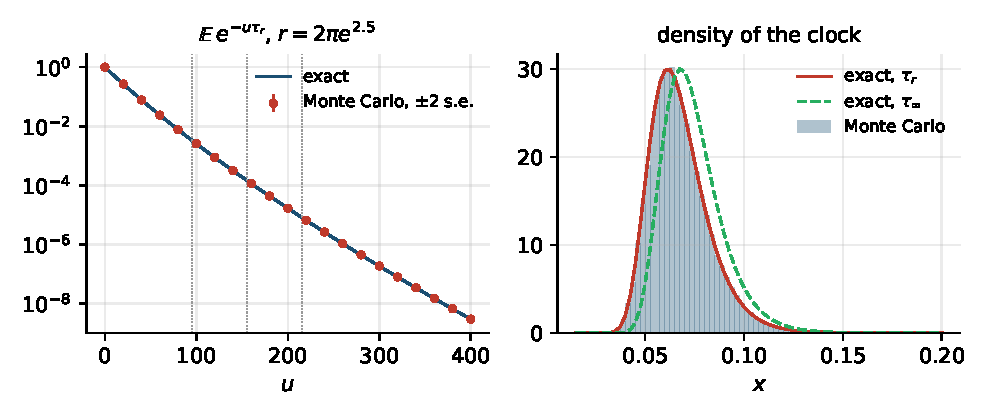
\includegraphics[width=\textwidth]{fig/biane_clock.pdf}
\caption{The clock from $R_0=2\pi e^{2.5}$. Left: $\E e^{-u\tau_{R_0}}$, exact and from the bridge corrected Monte Carlo with two standard errors, on a logarithmic scale; the dotted lines mark the first three Thorin atoms $\nu_1^2=95.4289$, $\nu_2^2=154.965$, $\nu_3^2=215.648$ of $\tau_\infty$. Right: the histogram of the corrected hitting times against the exact densities of $\tau_{R_0}$ and of $\tau_\infty$, by Talbot inversion. Drawn by \texttt{biane\_figs.py} from \texttt{biane\_clock.json}.}
\label{fig:biane:clock}
\end{figure}

The cosine dictionary \eqref{rz:eq:cosdict} turns each Thorin measure of this section into a L\'evy measure of the reciprocal transform, in the variable conjugate to the square root of the energy: a Thorin atom at $z$ becomes the exponential rate $\sqrt z$ when the energy is written $\lambda^2$, and $\sqrt{2z}$ when it is written $\lambda^2/2$, as for Brownian hitting times. Biane's measures give two classical L\'evy measures, and P\'olya's index side measure gives a wave trace.

\begin{proposition}\label{prop:biane:sin2}
For real $\lambda$, $a>0$, $c>0$ and $\ell>0$,
\begin{gather*}
2\log\frac{\sinh\lambda a}{\lambda a}=\int_0^\infty(1-\cos\lambda v)\,\frac{4\,dv}{v\,(e^{\pi v/a}-1)},\\
\ell\big(\sqrt{c^2+\lambda^2}-c\big)=\int_0^\infty(1-\cos\lambda v)\,\frac{2\ell c}\pi K_1(cv)\,\frac{dv}v,\\
\log\frac{K_\lambda(2\pi)}{K_0(2\pi)}=\int_0^\infty4\sin^2\Big(\frac{\lambda v}2\Big)\,\Theta_P(v)\,\frac{dv}v,\qquad\Theta_P(v)=\sum_{n\ge1}e^{-\nu_nv}=\operatorname{tr}e^{-v\sqrt{A_P}} .
\end{gather*}
The left sides are $-\log\E e^{-\lambda^2W/2}$ for $W=J_a+J'_a$ and $W=H^{(c)}_\ell$, and $-\log\E e^{-\lambda^2T_P}$.
\end{proposition}

\begin{proof}
By Frullani's integral, $\log(1+\lambda^2/\beta^2)=\int_0^\infty(1-\cos\lambda v)\,2e^{-\beta v}dv/v$. For $W=J_a+J'_a$ the Thorin measure $2\sum_n\delta_{\pi^2n^2/2a^2}$ of Section~\ref{sec:biane:hit} gives, at $u=\lambda^2/2$, the rates $\beta=\pi n/a$ with weight $2$, and $\sum_ne^{-\pi nv/a}=(e^{\pi v/a}-1)^{-1}$. For $H^{(c)}_\ell$ the density $\ell\{\pi\sqrt{2z-c^2}\}^{-1}$ on $z>\frac{c^2}2$ becomes, under $\beta=\sqrt{2z}$, the measure $\ell\beta\,d\beta/(\pi\sqrt{\beta^2-c^2})$ on $(c,\infty)$, and $\int_c^\infty e^{-\beta v}\beta(\beta^2-c^2)^{-1/2}d\beta=cK_1(cv)$. For $T_P$ take Theorem~\ref{thm:biane:indexP} at $u=\lambda^2$, with rates $\nu_n$, and use $1-\cos=2\sin^2(\cdot/2)$.
\end{proof}

\texttt{biane\_polya.py} checks the first two identities at $\lambda=1.7$, $a=1$, $c=1$, $\ell=0.8$, with the values $0.8845634041934098$ and $0.7778466338652816$ both ways. The Bessel clock has the Planck measure, a geometric superposition of the frequencies $\pi n/a$, and the drifted clock has the Macdonald measure, absolutely continuous because its spectrum is. The dictionary acts on Thorin measures, not on Biane's L\'evy measures in the time variable, which are heat traces. For P\'olya's function the third identity is the exact analogue of the L\'evy Khintchine form of $\xi(\frac12)/\xi(\frac12+u)$ in Section~\ref{sm:sec:poisson}, with the Poisson trace $K_{1/2}$ replaced by the wave trace $\Theta_P$ of the selfadjoint operator $A_P$, which is completely monotone with no hypothesis. In the variable $\theta$, where the zeros of $P$ are $2\nu_n$, the trace is $K^P(y)=\Theta_P(2y)=\sum_ne^{-2\nu_ny}$, and $\log(K_{\lambda/2}(2\pi)/K_0(2\pi))=\int_0^\infty4\sin^2(\lambda y/2)K^P(y)\,dy/y$ has the form of the formula for $\xi$ with $K^P$ in place of $K_{1/2}$; Section~\ref{sec:biane:cm} compares the two traces. At $\lambda=1.7$ the left side of the third identity is $0.2132910704$; the sum over all $1516$ zeros $\nu_n\le1000$ with the tail of Table~\ref{tab:biane:products} differs from it by $3\times10^{-10}$, and the $101$ zeros $\nu_n<120$ with the plain density, as in the note, give $0.2133932327$.

\subsection{Rindler modes and a Klein Gordon criterion}\label{sec:biane:kg}

The clock of Theorem~\ref{thm:biane:clock} lives in the Euclidean plane. Undoing the Wick rotation of the angle gives a Lorentzian picture in which P\'olya's function is a standard object of quantum field theory, and which isolates the structural reason for the reality of its zeros. Put
\[
F(x,w)=\exp(-e^x\cosh w),\qquad\text{so that}\qquad K_\mu(e^x)=\frac12\int_{\R}F(x,w)\,e^{\mu w}\,dw .
\]
Since $\partial_x^2F=(e^{2x}\cosh^2w-e^x\cosh w)F$ and $\partial_w^2F=(e^{2x}\sinh^2w-e^x\cosh w)F$,
\[
\Big(\frac{\partial^2}{\partial x^2}-\frac{\partial^2}{\partial w^2}-e^{2x}\Big)F=0 .
\]
In the coordinates $X_1=e^x\cosh w$, $X_0=e^x\sinh w$ of the Rindler wedge $X_1>|X_0|$, in which $\rho=e^x$ is the proper distance from the edge of the wedge and $w$ the rapidity, $\partial_{X_1}^2-\partial_{X_0}^2=e^{-2x}(\partial_x^2-\partial_w^2)$, so the equation is $(\partial_{X_1}^2-\partial_{X_0}^2-1)F=0$ with $F=e^{-X_1}$: the Klein Gordon equation of unit mass in $1+1$ dimensional Minkowski space, solved by a plane wave. The index $\mu$ is the eigenvalue of the boost generator $\partial_w$, and $K_{i\omega}(\rho)$ is the Rindler mode of boost frequency $\omega$ \cite{Fulling73}. The zeros of $P(\theta)=K_{i\theta/2}(2\pi)$ are therefore, with $\theta=2\omega$, the boost frequencies of the normal modes of a unit mass scalar field in the Rindler wedge with a Dirichlet mirror on the hyperbola $\rho=2\pi$, the configuration of 't Hooft's brick wall model of a black hole horizon \cite{tHooft85}. Biane's Dirac system of Section~\ref{sec:biane:zeros} is the corresponding Dirac field, close to the Rindler space models of Sierra for the Hamiltonian $xp$ \cite{Sierra14}.

The Wick rotation $w=i\phi$ turns the wedge into the Euclidean plane in polar coordinates $(\rho,\phi)$, the boost into a rotation, the Klein Gordon operator into $\Delta-1$, and the plane wave $e^{-X_1}$ into $e^{-\rho\cos\phi}$, which is harmonic for $\frac12(\Delta-1)$, the generator of planar Brownian motion killed at rate $\frac12$ of Theorem~\ref{thm:biane:clock}. The boost frequency becomes the angular momentum $\mu$, and the radial operator $\frac12(\partial_\rho^2+\rho^{-1}\partial_\rho-\mu^2/\rho^2-1)$ carries the index as the centrifugal term that the Feynman Kac weight of the clock produces. The energy of Biane's dictionary, the rapidity of the Rindler picture and the index of the clock are three readings of one rotation, the last row of Table~\ref{tab:biane:wick}. The structure that makes the zeros of $P$ real can be stated for a general even kernel.

\begin{theorem}[A Klein Gordon criterion]\label{thm:biane:kg}
Let $g$ be even, positive and continuous with $\int g(w)e^{c|w|}dw<\infty$ for every $c$, and $G(t)=\int g(w)e^{itw}dw$. Suppose that there are $x_0\in\R$, a real continuous function $V$ on $[x_0,\infty)$ bounded below, and $F\in C^2([x_0,\infty)\times\R)$ such that
\begin{enumerate}
\item[(a)] $(\partial_x^2-\partial_w^2-V(x))F=0$ and $F(x_0,\cdot)=g$;
\item[(b)] $F$ and its partial derivatives of order at most two are $O(e^{-c|w|})$ for every $c>0$, uniformly for $x$ in compact subsets of $[x_0,\infty)$, and $\Psi_\mu(x)=\int F(x,w)e^{\mu w}dw$ lies in $L^2((x_0,\infty))$ for every $\mu\in\C$;
\item[(c)] $\Psi_\mu$ is not identically zero for any $\mu\in\C$.
\end{enumerate}
Then every zero of $G$ is real, and its square is an eigenvalue of $-\frac{d^2}{dx^2}+V$ on $[x_0,\infty)$ with a Dirichlet condition at $x_0$.
\end{theorem}

\begin{proof}
By (b), $\Psi_\mu$ is twice differentiable under the integral sign, and two integrations by parts in $w$, whose boundary terms vanish, give $\Psi_\mu''=\int(\partial_w^2F+VF)e^{\mu w}dw=(\mu^2+V)\Psi_\mu$. Since $V$ is bounded below, the operator $-\frac{d^2}{dx^2}+V$ is in the limit point case at $\infty$, and its Dirichlet realisation at $x_0$ is selfadjoint. If $G(t)=0$, then $\Psi_{it}(x_0)=G(t)=0$ by (a), and by (b) and (c) $\Psi_{it}$ is an eigenfunction with eigenvalue $-(it)^2=t^2$, which is therefore real. So $t$ is real or purely imaginary, and $t=-i\mu$ with real $\mu$ is excluded because $G(-i\mu)=\int g(w)e^{\mu w}dw>0$.
\end{proof}

For P\'olya's function the hypotheses hold in the rapidity variable $w=2u$: with $g(w)=e^{-2\pi\cosh w}$, $G(t)=2K_{it}(2\pi)=2P(2t)$, $V(x)=e^{2x}$, $x_0=\log2\pi$, $F=\exp(-e^x\cosh w)$ and $\Psi_\mu(x)=2K_\mu(e^x)$, and the theorem gives Proposition~\ref{prop:biane:liouville}(ii) again. \texttt{biane\_polya.py} checks the equation for $F$ at $(x,w)=(0.7,0.4)$, with residual $-5.7\times10^{-42}$ at $40$ digits. The criterion says that the reality of the zeros of an even Fourier transform follows from embedding its kernel as the boundary value of a field that satisfies a Klein Gordon equation with a real, time independent potential, which decays fast enough in the rapidity.

For $\Xi$ the corresponding object would be such an extension of $\Phi$, and it would prove RH (Question~\ref{q:biane:kg}). The scaling matters. For $P$ the eigenvalues of $A_P$ are $\nu_n^2=\theta_n^2/4$, and the function whose zeros they are, as a function of the spectral parameter $\mu$ at the boundary $x_0$, is the Jost function $\mu\mapsto\Psi_\mu(x_0)=2K_\mu(2\pi)=2P(-2i\mu)$. A potential asymptotic to $e^{2x}$ at $+\infty$ has the Weyl law of Proposition~\ref{prop:biane:phase}, which matches the zeros of $\Xi$ only in the same scaling, $g(w)=\Phi(w/2)$ and $G(t)=2\Xi(2t)$, and then the Jost function is $\mu\mapsto2\Xi(-2i\mu)=2\xi(\frac12+2\mu)$. The note \cite{P26bia} proposes $\mu\mapsto\xi(\frac12+\mu)$, which corresponds to the eigenvalues $\gamma^2$, whose density is half that of the Weyl law of $e^{2x}$ (a potential growing like $e^{4x}$ would match them). Inverse spectral theory reconstructs an operator from its eigenvalues and norming constants, a potential in the forms of Gelfand and Levitan or of Marchenko and a string in Krein's form, and under RH and the simplicity of the zeros Krein's theory realises the eigenvalues $\gamma^2/4$ (Section~\ref{sec:ch18:kent}); the content of the question is that the operator be of the form $-\frac{d^2}{dx^2}+V$ and that $V$ admit a Klein Gordon solution whose boundary value is $\Phi(w/2)$, which is a statement about the whole function $\xi$ and not only about its zeros.

\subsection{The de Bruijn Newman flow of \texorpdfstring{$P$}{P} against that of \texorpdfstring{$\Xi$}{Xi}}\label{sec:biane:flow}

For real $t$ put
\begin{gather*}
P_t(\theta)=\int_{\R}e^{tu^2/4}e^{-2\pi\cosh2u}\,e^{i\theta u}\,du,\\
\Xi_t(\theta)=\int_{\R}e^{tu^2/4}\,\Phi(u)\cos(\theta u)\,du=8H_t(2\theta),
\end{gather*}
so that $P_0=P$, $\Xi_0=\Xi$, and $t$ is the time of the de Bruijn Newman flow in the normalisation of Section~\ref{sec:ch21:flow}. Decreasing $t$ is the direction in which real zeros can be lost: RH is the statement that $\Xi_t$ keeps only real zeros down to $t=0$, and by the theorem of Rodgers and Tao \cite{RodgersTao} it has nonreal zeros for every $t<0$. For P\'olya's kernel the analogous constant is finite.

\begin{proposition}\label{prop:biane:lambdaP}
There is a constant $\Lambda_P$ with $-\infty<\Lambda_P\le0$ such that $P_t$ has only real zeros if and only if $t\ge\Lambda_P$.
\end{proposition}

\begin{proof}
Let $S$ be the set of $t$ for which $P_t$ has only real zeros. By Proposition~\ref{prop:biane:liouville}, $0\in S$. If $t\in S$ and $t'>t$, then $t'\in S$ by de Bruijn's theorem on the Gaussian factor $e^{\lambda u^2}$, $\lambda>0$ \cite[Theorem~13]{deBruijn}, which applies to the kernel $e^{tu^2/4}e^{-2\pi\cosh2u}$ because it is $O(e^{-|u|^b})$ for every $b>2$. If $t_k\in S$ decrease to $t$, then $P_{t_k}\to P_t$ locally uniformly on $\C$ by dominated convergence, with $|e^{t_ku^2/4}e^{i\theta u}|\le e^{t_1u^2/4}e^{|\im\theta||u|}$, and $P_t(0)>0$, so by Hurwitz's theorem every zero of $P_t$ is a limit of real zeros and $t\in S$. Hence $S=[\Lambda_P,\infty)$ with $\Lambda_P\in[-\infty,0]$. Suppose $\Lambda_P=-\infty$. Then, for the even probability measure $\rho$ with density $e^{-2\pi\cosh2u}/K_0(2\pi)$, the Fourier transform of $e^{\lambda u^2}\rho(du)$ has only real zeros for every real $\lambda$, and by Newman's theorem \cite{Newman1976}, \cite[Theorem 10]{NewmanWu20}, $\rho$ is either $\frac12(\delta_{u_0}+\delta_{-u_0})$ or has a density $Ku^{2m}\exp(-\alpha u^4-\beta u^2)\prod_j(1+u^2/a_j^2)e^{-u^2/a_j^2}$, with $K>0$, $m\ge0$ an integer, $a_j>0$, $\sum_ja_j^{-4}<\infty$, and $\alpha>0$, or $\alpha=0$ and $\beta+\sum_ja_j^{-2}>0$. The inequality $(1+y)e^{-y}\ge e^{-y^2/2}$ for $y\ge0$ bounds such a density below by $Ku^{2m}\exp(-[\alpha+\sum_j\frac1{2a_j^4}]u^4-\beta u^2)$, while $e^{-2\pi\cosh2u}$ decays faster than $e^{-Cu^4}$ for every $C$. This contradiction gives $\Lambda_P>-\infty$.
\end{proof}

The proof is Newman's proof that $\Lambda>-\infty$ \cite{Newman1976}, Theorem~9 of \cite{NewmanWu20}, which uses only the fact that the kernel decays faster than $e^{-Cu^4}$ for every $C$; it applies verbatim to $\Phi^*$, and to every even, positive kernel with that decay whose Fourier transform has only real zeros. The note \cite{P26bia} conjectures $\Lambda_P=-\infty$, on the evidence of the computation below; Proposition~\ref{prop:biane:lambdaP} shows that the conjecture is false. The computation is still informative, because it shows how differently the two flows behave in the range that can be followed.

\texttt{biane\_flow.py} computes both transforms by the trapezoid rule with step $1/250$ on $[0,2]$ at $90$ digits. The kernels are analytic in $|\im u|<\pi/4$ (the kernel of $P_t$ is entire) and below $10^{-68}$ beyond $u=2$, and at $t=0$ the sums reproduce Arb's $K_{i\theta/2}(2\pi)$ at $\theta=10$, $30$, $60$, $90$ and mpmath's $\Xi$ at $\theta=14.134725$, $50$, $90$ with relative errors between $3.5\times10^{-62}$ and $1.4\times10^{-45}$, the largest at $\theta=90$. The real zeros in $(0,90)$ are located by sign changes on a grid of step $0.05$ and refined, for $t=0,-0.5,\dots,-20$ and $t=-21,\dots,-60$. Table~\ref{tab:biane:flow} and Figure~\ref{fig:biane:flow} show the result. The real zeros of $\Xi_t$ in the window fall from $25$ at $t=0$ to $17$ at $t=-2$, $11$ at $t=-4$, $7$ at $t=-8$ and $2$ at $t=-40$, and they are lost in pairs, neighbouring zeros colliding and leaving the axis: the first collisions in the window, as $t$ decreases, are those of the census of Section~\ref{sec:ch21:hankel}, beginning with $(\gamma_{24},\gamma_{25})$ at $t=-1.144$ and height $88.47$ near the top of the window. The pair $(\gamma_4,\gamma_5)=(30.42,32.94)$ has gone by $t=-4$, and the pair $(\gamma_2,\gamma_3)$ by $t=-15$, after which the first zero is isolated. For $P_t$ nothing of the kind occurs down to $t=-60$: every real zero moves monotonically upward, the first from $19.538$ at $t=0$ to $51.881$ at $t=-60$, and the number in the window falls only as zeros leave it through $\theta=90$: from each time of the grid to the next, every zero increases and the count never increases.

\begin{table}[htbp]
\centering\small
\begin{tabular}{rrlrl}
\toprule
$t$ & $P_t$: zeros & first zero & $\Xi_t$: zeros & first zeros\\
\midrule
$0$ & $24$ & $19.538$ & $25$ & $14.135$, $21.022$, $25.011$\\
$-1$ & $23$ & $19.938$ & $25$ & $14.426$, $21.403$, $25.302$\\
$-2$ & $23$ & $20.342$ & $17$ & $14.719$, $21.793$, $25.589$\\
$-4$ & $23$ & $21.163$ & $11$ & $15.311$, $22.600$, $26.144$\\
$-6$ & $23$ & $22.002$ & $9$ & $15.911$, $23.452$, $26.667$\\
$-8$ & $22$ & $22.857$ & $7$ & $16.518$, $24.365$, $27.139$\\
$-10$ & $22$ & $23.730$ & $7$ & $17.133$, $25.378$, $27.518$\\
$-15$ & $21$ & $25.987$ & $5$ & $18.695$, $44.574$, $58.128$\\
$-20$ & $20$ & $28.353$ & $5$ & $20.290$, $46.563$, $60.344$\\
$-25$ & $19$ & $30.832$ & $5$ & $21.911$, $48.426$, $62.880$\\
$-30$ & $18$ & $33.428$ & $3$ & $23.551$, $50.245$, $89.062$\\
$-40$ & $17$ & $38.989$ & $2$ & $26.866$, $53.858$\\
$-50$ & $15$ & $45.098$ & $2$ & $30.202$, $57.488$\\
$-60$ & $13$ & $51.881$ & $2$ & $33.539$, $61.145$\\
\bottomrule
\end{tabular}
\caption{The real zeros in $(0,90)$ of $P_t$ and $\Xi_t$ along the de Bruijn Newman flow: their numbers, the first zero of $P_t$ and the first three of $\Xi_t$. Computed by \texttt{biane\_flow.py}.}
\label{tab:biane:flow}
\end{table}

\begin{figure}[htbp]
\centering
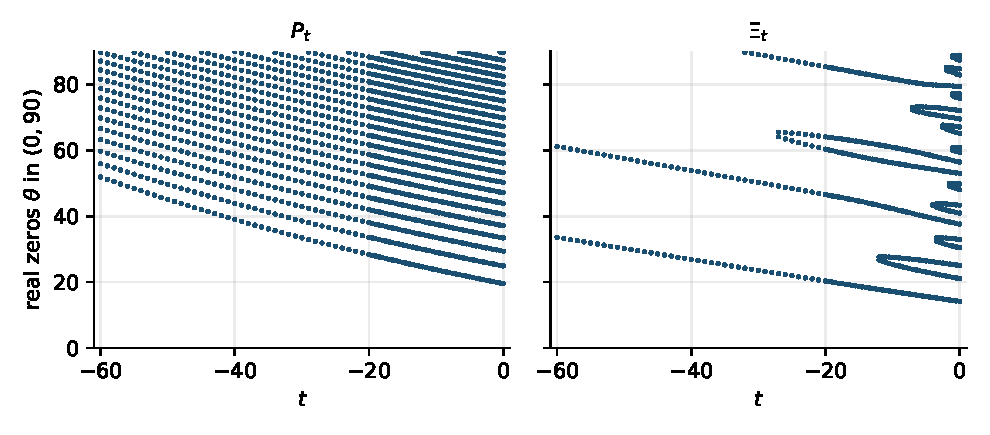
\includegraphics[width=\textwidth]{fig/biane_flow.pdf}
\caption{The real zeros in $(0,90)$ of $P_t$ (left) and of $\Xi_t$ (right) for $-60\le t\le0$, on the grid of Table~\ref{tab:biane:flow} (step $0.5$ above $t=-20$, step $1$ below). The zeros of $P_t$ drift upward and leave the window one at a time; those of $\Xi_t$ collide in pairs. Drawn by \texttt{biane\_figs.py} from \texttt{biane\_flow.json}.}
\label{fig:biane:flow}
\end{figure}

Sign changes count only real zeros, so the script also counts all zeros in the box $0.5\le\re\theta\le60.3$, $|\im\theta|\le3$ by the argument principle, on a contour of step $0.04$ halved wherever the argument changes by more than $0.5$ between neighbours; the largest change that remains is $0.36$. For $P_t$ the box holds $12$, $11$, $8$ and $3$ zeros at $t=0$, $-10$, $-30$ and $-60$, all of them real. For $\Xi_t$ it holds $13$, $12$ and $12$ zeros at $t=0$, $-2$ and $-4$, of which $13$, $10$ and $8$ are real: one conjugate pair has appeared by $t=-2$ and two by $t=-4$. Three of the collisions below height $60$, those listed in the note \cite{P26bia}, are located by bisection in $t$ for the disappearance of two sign changes and then by Newton's method for the double zero $\Xi_t=\partial_\theta\Xi_t=0$ in $(\theta,t)$:
\begin{gather*}
(\gamma_9,\gamma_{10}):\ t_c=-1.877909073,\ \theta_c=49.66423465;\\
(\gamma_4,\gamma_5):\ t_c=-3.954792524,\ \theta_c=33.09873381;\\
(\gamma_2,\gamma_3):\ t_c=-12.49451313,\ \theta_c=27.3212277 .
\end{gather*}
The first agrees with the census of Section~\ref{sec:ch21:hankel} ($-1.87791$ at height $49.664$); the other two lie below its range $[-2.05,0]$. The note presents the three as the first collisions below height $60$, but the computation, on its grid of step $0.5$ in $t$, shows a fourth before $t=-12.5$: the zeros $\gamma_7$ and $\gamma_8$ are at $43.263$ and $43.522$ at $t=-4$ and have left the axis at $t=-4.5$, and the isolated pair estimate of Section~\ref{sec:ch21:flow} puts their collision at about $t=-4.03$, just after that of $(\gamma_4,\gamma_5)$, although they are the closer pair at $t=0$ ($2.408$ apart, against $2.510$). The pair $(\gamma_9,\gamma_{10})$ is the closest pair below height $60$, at distance $1.769$, and its isolated pair estimate $-\frac12(1.769)^2=-1.565$ of Section~\ref{sec:ch21:flow} is again an overestimate of the collision time, the neighbours delaying the collision. In the variable $\theta$ a simple zero moves by
\[
\frac{d\theta_k}{dt}=\frac{\partial_\theta^2F_t(\theta_k)}{4\,\partial_\theta F_t(\theta_k)}=\frac12\sum_{j\ne k}\frac1{\theta_k-\theta_j},
\]
for $F_t=P_t$ and for $F_t=\Xi_t$, which is the equation of motion of Section~\ref{sec:ch21:flow} with $z=2\theta$. At $t=0$ the formula gives $-0.39798088$ for the first zero of $P$ and $-0.28981529$ for the first zero of $\Xi$, and central differences in $t$ with step $10^{-3}$ give the same eight digits. As $t$ decreases every two zeros attract each other, and since the zeros above a given zero are more numerous and denser than those below it, the net pull is upward, which is why both sets of zeros rise; a pair collides when its mutual attraction overcomes the difference of the pulls of all the other zeros on its two members. For $P$ the configuration is regular enough that this does not happen in the window.

The mean motion can be predicted. For $\theta>4\pi$ the integral $P(\theta)$ is dominated by the conjugate saddle points $u_\pm=\pm\frac x2+\frac{i\pi}4$ of $i\theta u-2\pi\cosh2u$, with $x=\operatorname{arccosh}(\theta/4\pi)$, where the exponent is $-\frac{\pi\theta}4\pm i(\frac12\theta x-2\pi\sinh x)$. So $P(\theta)$ is $e^{-\pi\theta/4}$ times a slowly varying amplitude times a cosine of phase $\varphi(\theta)=\frac12\theta x-2\pi\sinh x$ plus a constant; since $\varphi'(\theta)=\frac x2$, the zeros have density $\frac x{2\pi}=\frac1{2\pi}\log\frac\theta{2\pi}+O(\theta^{-2})$. To first order in $t$ the factor $e^{tu^2/4}$ adds to the phase the imaginary part $\frac{\pi t}{16}x$ of $\frac t4u_+^2$, so the number of zeros below a fixed height changes at the rate $\frac x{16}$ per unit of $t$, and each zero moves with
\[
\frac{d\theta}{dt}\approx-\frac{x/16}{x/2\pi}=-\frac\pi8,
\]
whatever its height. The equation of motion gives the same value: with the density $\frac1{2\pi}\log\frac{|\theta|}{2\pi}$ on both half lines, $\frac12\sum_{j\ne k}(\theta_k-\theta_j)^{-1}$ becomes $\frac1{4\pi}$ times the principal value integral of $\log|s|/(\theta_k-s)$, which is $-\frac{\pi^2}2$ for $\theta_k>0$. Over $-0.5\le t\le0$ the $24$ real zeros of $P$ in the window rise at mean speeds that decrease with the height from $0.3990$ (the first zero) to $0.3949$ (the last), towards $\pi/8=0.3927$, while the $25$ zeros of $\Xi$ rise at speeds between $0.0040$, for $\gamma_{25}$, held back by $\gamma_{24}$, which is closing on it, and $0.7350$, for $\gamma_{19}$, which is closing on $\gamma_{20}$, with mean $0.3647$ (\texttt{biane\_figs.py}). The zeros of $P$ move almost as a rigid block; those of $\Xi$ fluctuate about the same mean motion, and the fast and slow members of the close pairs are the ones that collide.

The regularity can be measured. In units of the local mean spacing $2\pi/\log(\theta/2\pi)$, taken at the midpoint of each gap, the smallest gap between consecutive real zeros in the window is
\begin{center}
\small
\begin{tabular}{lllll}
\toprule
$t$ & $0$ & $-10$ & $-30$ & $-60$\\
\midrule
$P_t$ & $1.002$ & $1.020$ & $1.059$ & $1.121$\\
$\Xi_t$ & $0.534$ & $0.490$ & three zeros left & two zeros left\\
\bottomrule
\end{tabular}
\end{center}
(\texttt{biane\_flow.py} and \texttt{biane\_figs.py}). The smallest gap of $P_t$ is always that between the two highest zeros of the window, at almost exactly the mean spacing, and it widens as $t$ decreases, while the smallest gaps of $\Xi_t$, $(59.347,60.832)$ at $t=0$ and $(25.378,27.518)$ at $t=-10$, shrink until the pairs collide. With the density taken at the lower end of each gap, as in the note \cite{P26bia}, the values are $0.968$, $1.014$, $1.053$, $1.115$ for $P_t$ and $0.531$, $0.476$ for $\Xi_t$, and the note's values agree with these to one unit in the third decimal; at $t=0$ the minimum for $P$ then moves to the first gap $(19.538,24.897)$, where the density changes fastest, which is an effect of the convention. The two functions have the same mean density of zeros, $\frac1{2\pi}\log\frac\theta{2\pi}$ (Proposition~\ref{prop:biane:phase}); what differs is the fluctuation, the sawtooth of a quantisation rule for $P$ against $S(T)$ for $\Xi$, whose close pairs (Lehmer pairs, Section~\ref{sec:ch21:collisions}) the flow pushes together.

\begin{remark}[One saddle pair against many]\label{rem:biane:saddle}
For fixed $t$ and large $\theta$ the integral $P_t(\theta)$ is governed by a single pair of complex saddle points of $i\theta u-2\pi\cosh2u+tu^2/4$, conjugate under $u\mapsto-\bar u$ because the kernel is real and even, so that $P_t(\theta)=2\re(Ae^{i\psi_t(\theta)})(1+o(1))$ with a monotone phase, as in P\'olya's asymptotics at $t=0$; heuristically, all but finitely many zeros of $P_t$ are then real for each fixed $t$. For $\Xi_t$ the large $\theta$ asymptotics is the Riemann Siegel expansion, with a number of interfering terms that grows with $\theta$, and the interference is $S(T)$. The note \cite{P26bia} suggests that a version of the saddle point argument uniform in $t$, with a finite computation, would prove $\Lambda_P=-\infty$. By Proposition~\ref{prop:biane:lambdaP} no such uniform version exists: as $t$ decreases below $\Lambda_P$, nonreal zeros appear, outside the box of the argument principle or at times the computation does not reach. The difference between $P$ and $\Xi$ is quantitative, the size of $|\Lambda_P|$ against $\Lambda=0$ under RH, not a difference between a finite and an infinite constant.
\end{remark}

In the language of Lee and Yang \cite{LeeYang} (Section~\ref{rz:sec:polya} and Proposition~\ref{rz:prop:newmanthorin}), the single spin law with density $e^{-2\pi\cosh2u}/K_0(2\pi)$ has the Lee and Yang property, since its moment generating function $K_{h/2}(2\pi)/K_0(2\pi)$ vanishes only at imaginary $h$; it is the ferromagnetic law $U$ of Section~\ref{sec:biane:index}. Newman's theorem says that this property survives every Gaussian factor $e^{-bu^2}$, $b>0$, only for two point laws and for the densities of the proof of Proposition~\ref{prop:biane:lambdaP}, which include the $\varphi^4$ laws $e^{-au^4-bu^2}$ that Simon and Griffiths realised as limits of Ising ferromagnets \cite{SimonGriffiths73}. The law with density proportional to $e^{-2\pi\cosh2u-bu^2}$ has the property exactly when its Fourier transform, a multiple of $P_{-4b}$, has only real zeros, that is when $b\le-\Lambda_P/4$. So the Simon Griffiths type construction for $e^{-2\pi\cosh2u-bu^2}$ at every real $b$ that the note proposes cannot exist.

\subsection{P\'olya's function and \texorpdfstring{$\Xi$}{Xi} side by side}\label{sec:biane:assess}

Table~\ref{tab:biane:compare} sets the two functions side by side. It follows the comparison in the note \cite{P26bia}, corrected in three rows: the index side clock of $\Xi$ exists with no hypothesis, the de Bruijn Newman constant of $P$ is finite, and the computation of the flow describes a window of heights and times, not the whole flow. The Wick rotation of Section~\ref{sec:biane:wick} relates the two entries of each of the second, third and fourth rows. Discreteness moves across the table: $P$ is continuous in the energy and discrete in the angular momentum, while $\Xi$ is discrete in the energy and, under RH, in the angular momentum.

\begin{table}[htbp]
\centering\small
\begin{tabular}{@{}p{0.20\textwidth}p{0.36\textwidth}p{0.36\textwidth}@{}}
\toprule
& P\'olya's $P(\theta)=K_{i\theta/2}(2\pi)$ & Riemann's $\Xi(\theta)$\\
\midrule
kernel & $e^{-2\pi\cosh2u}$, \eqref{eq:biane:P} & $\Phi(u)$, \eqref{eq:ch2:Phi}\\
hitting time & $H^{(\sqrt{2\pi})}_{\sqrt{2\pi}}$, Brownian motion with drift (Proposition~\ref{prop:biane:mellin}) & $\frac\pi2S_2$, three dimensional Bessel process, \eqref{bp:eq:bpy}\\
symmetric space & $\mathbb H^3=SL_2(\C)/SU(2)$ & $SU(2)\cong S^3$\\
Thorin measure of the hitting time (energy) & continuous: $\sigma_2$ for $H^{(1)}_1$ & discrete: $2\pi\sigma_1$ for $\pi^2S_2$ (Theorem~\ref{thm:biane:dict})\\
index side Thorin measure (angular momentum) & $\sum_n\delta_{\nu_n^2}$, a theorem (Theorem~\ref{thm:biane:indexP}) & $\sum_\gamma\delta_{\gamma^2}$ if and only if RH (Proposition~\ref{prop:rigid})\\
index side clock & $\tau_\infty$, a hitting time of an explicit diffusion (Theorem~\ref{thm:biane:clock}) & a random time $T$ (Theorem~\ref{thm:ch12:idsd}); no diffusion is known (Question~\ref{q:biane:radial})\\
trace of the sine squared form & $\Theta_P=\operatorname{tr}e^{-v\sqrt{A_P}}$, completely monotone (Proposition~\ref{prop:biane:sin2}) & $K_{1/2}$, completely monotone if and only if RH (Corollary~\ref{sm:cor:poisson})\\
operator for the zeros & $-\frac{d^2}{dx^2}+e^{2x}$ on $[\log2\pi,\infty)$ (Proposition~\ref{prop:biane:liouville}) & not known\\
Klein Gordon extension & $\exp(-e^x\cosh w)$ (Theorem~\ref{thm:biane:kg}) & not known (Question~\ref{q:biane:kg})\\
de Bruijn Newman constant & $-\infty<\Lambda_P\le0$ (Proposition~\ref{prop:biane:lambdaP}) & $\Lambda\ge0$ \cite{RodgersTao}; RH if and only if $\Lambda=0$\\
real zeros in $(0,90)$ for $-60\le t\le0$ & no collision; mean speeds $0.395$ to $0.399$ on $[-0.5,0]$ & collisions in pairs from $t=-1.144$; mean speeds $0.004$ to $0.735$ on $[-0.5,0]$\\
\bottomrule
\end{tabular}
\caption{P\'olya's function and $\Xi$. Apart from the computations of the last row, the left column is a list of theorems; in the right column the entries that concern the zeros are equivalent to RH or open.}
\label{tab:biane:compare}
\end{table}

The statements about $\Xi$ in the right column and their relatives, Proposition~\ref{prop:rigid}, Corollary~\ref{sm:cor:poisson}, Proposition~\ref{rz:prop:lpthorin} and the GGC form of the clock $T$ discussed after Corollary~\ref{cor:biane:bm}, are proved by Hadamard factorisation, Bernstein's theorem and integral identities. No property of the primes enters their proofs, and none could, since each is an equivalence between two statements about the zeros of one entire function: they reorganise RH, as Section~\ref{ch:open} says of the programme as a whole, and do not approach it. The left column shows that the reorganisation is coherent, since for $P$ every entry is a theorem; but the proofs of the entries on the left that concern the zeros all go through the selfadjoint operator $A_P$, which is exactly what the right column lacks.

The de Bruijn Newman constant explains why a whole family of arguments cannot succeed. The note \cite{P26bia} proves part (a) of the following proposition; part (b) is the strengthening that Newman's theorem gives, and it changes the reading of part (a).

\begin{proposition}\label{prop:biane:damping}
Let $\mathcal P$ be a property of even, positive, integrable kernels such that
\begin{enumerate}
\item[(i)] if $\mathcal P(g)$ holds, then $\int g(u)e^{i\theta u}du$ has only real zeros, and
\item[(ii)] there is $\varepsilon>0$ such that $\mathcal P(g)$ implies $\mathcal P(e^{-\varepsilon u^2/4}g)$.
\end{enumerate}
\begin{enumerate}
\item[(a)] If (ii) holds for $g=\Phi$, then $\mathcal P(\Phi)$ is false.
\item[(b)] If (ii) holds for all $g$ with the same $\varepsilon$, then $\mathcal P(g)$ is false for every kernel $g$ that is $O(e^{-|u|^b})$ for some $b>2$ and satisfies $g(u)e^{Cu^4}\to0$ as $|u|\to\infty$ for every $C$; in particular $\mathcal P$ fails for $\Phi$, for $\Phi^*$ and for $e^{-2\pi\cosh2u}$.
\end{enumerate}
\end{proposition}

\begin{proof}
(a) If $\mathcal P(\Phi)$ held, then by (ii) and (i) the transform of $e^{-\varepsilon u^2/4}\Phi$, which is $\Xi_{-\varepsilon}$ of Section~\ref{sec:biane:flow}, would have only real zeros, so $\Lambda\le-\varepsilon<0$, against the theorem of Rodgers and Tao \cite{RodgersTao}. (b) If $\mathcal P(g)$ held, then by induction $\mathcal P(e^{-k\varepsilon u^2/4}g)$ would hold for $k=0,1,2,\dots$, so the transform of $e^{-k\varepsilon u^2/4}g$ would have only real zeros for each $k$. This kernel is again $O(e^{-|u|^b})$, so by de Bruijn's theorem \cite[Theorem~13]{deBruijn} the transform of $e^{tu^2/4}g$ would have only real zeros for every $t\ge-k\varepsilon$, and hence for every real $t$. By Newman's theorem, as in the proof of Proposition~\ref{prop:biane:lambdaP}, $g/\int g$ would be a density of the form given there, which is bounded below by $Ku^{2m}\exp(-C'u^4-\beta u^2)$ for some $C'$, against the decay of $g$.
\end{proof}

Part (a) uses the theorem of Rodgers and Tao and concerns $\Phi$ alone. Part (b) uses only de Bruijn's theorem and Newman's theorem of 1976, and it shows that the obstruction has nothing to do with the position of $\Phi$ on the boundary of the class of kernels with real zeros: a property that survives a fixed amount of damping for all kernels fails for $P$ as well, although the zeros of $P$ are real for a structural reason, the selfadjointness of $A_P$. So the reading in the note, that P\'olya's kernel tolerates every Gaussian damping, that $P$ has slack and $\Xi$ none, is to be replaced by a quantitative one: $P$ has the finite slack $|\Lambda_P|$, whose size is not known, and $\Xi$ has none if RH holds. Part (b) also limits what the proposition excludes. The note lists among the excluded arguments a ferromagnetic or Lee and Yang construction and a Simon Griffiths representation. The Lee and Yang property of a single spin law is preserved by the ferromagnetic factor $e^{bu^2}$, $b>0$, which runs the flow forward, but by (b) it is not preserved by a fixed damping except on Newman's class. A Lee and Yang representation of the law with density proportional to $\Phi$, which is equivalent to RH (Proposition~\ref{rz:prop:newmanthorin}), is therefore not excluded by the proposition, and neither is a Simon Griffiths type representation of that law. What the proposition excludes is a construction with room to spare, one that would apply to $e^{-\varepsilon u^2/4}\Phi$ as well. The criteria of this section are positivity statements equivalent to RH, of the kind whose history Section~\ref{st:sec:wp5} recalls with the example of Conrey and Li \cite{CL00}; their value here is as a dictionary, not as a plan.

Three questions raised by the note are not equivalences and can be studied without assuming what is to be proved. The first two ask for an object, a diffusion or a potential, not for the zeros, and part (b) does not apply to them, because the existence of such an object is not preserved by a fixed Gaussian damping of every kernel: for $P$ it is lost at every $t<\Lambda_P$, where $P_t$ has nonreal zeros. The third is a question about an explicit kernel with no arithmetic in it, and it measures the slack of P\'olya's function. A fourth concerns the interpolation between the two clocks of Section~\ref{sec:biane:wick}.

\begin{question}\label{q:biane:radial}
Is there a diffusion on a half line, with an entrance boundary, whose hitting time of a level from the entrance boundary has the Laplace transform $\xi(\frac12)/\xi(\frac12+2\sqrt u)$, the transform of the clock $T$ of Theorem~\ref{thm:ch12:idsd} scaled by $4$, as $\tau_\infty$ has the transform $K_0(2\pi)/K_{\sqrt u}(2\pi)$ in Theorem~\ref{thm:biane:clock}? By Kent's theorem \cite{Kent80} such a hitting time is $\sum_ne_n/\lambda_n$ over the Dirichlet eigenvalues $\lambda_n>0$ of the generator, so a positive answer implies RH; under RH and the simplicity of the zeros, Krein's inverse spectral theory gives a generalised diffusion with the eigenvalues $\gamma^2/4$ (Section~\ref{sec:ch18:kent}). The question asks for one constructed without RH, for example as a perturbation of the diffusion $X$ of Section~\ref{sec:biane:index}, whose potential $e^{2x}$ has the right Weyl law.
\end{question}

\begin{question}\label{q:biane:kg}
Does $g(w)=\Phi(w/2)$ admit a Klein Gordon extension in the sense of Theorem~\ref{thm:biane:kg}, with a real potential $V$ asymptotic to $e^{2x}$ at $+\infty$? By the theorem a positive answer implies RH. Under RH the question asks whether $\mu\mapsto2\xi(\frac12+2\mu)$ is, up to normalisation, the Jost function of such a potential whose Klein Gordon solution has the boundary value $g$. A first numerical step is to reconstruct a potential from the first few thousand ordinates and a choice of norming constants by the method of Gelfand and Levitan or of Marchenko, and to test whether it is stable under truncation and close to $e^{2x}$.
\end{question}

\begin{question}\label{q:biane:lambda}
What is the de Bruijn Newman constant $\Lambda_P$ of P\'olya's function, and that of $\Xi^*$, which is also finite and at most $0$ by the proof of Proposition~\ref{prop:biane:lambdaP}? At what height do the first nonreal zeros of $P_t$ appear as $t$ decreases through $\Lambda_P$, and do they appear, as for $\Xi_t$, through the collision of two real zeros?
\end{question}

\begin{question}\label{q:biane:curv}
Is there a one parameter family of laws joining the drifted first passage time and the sum of two Bessel hitting times, each with a reciprocal symmetry that encodes a functional equation, as $\tau\mapsto1/\tau$ does for $H$ in Proposition~\ref{prop:biane:mellin}(i) and Jacobi's transformation does for $S_2$, along which the index side Thorin measure can be followed? The curvature family of Proposition~\ref{prop:biane:skappa} is an Esscher tilt and breaks the symmetry. Positivity of the index side Thorin measure at the Bessel end is RH.
\end{question}
